%\documentclass[review,number,sort&compress]{elsarticle} 
% this is the default style (single column!) for submission of
% your paper

\documentclass[final,5p,times,twocolumn]{elsarticle} 
% this is the double column style for checking the final length 
% of your paper in the proceedings

\usepackage{lineno}
\linenumbers

%% if you use PostScript figures in your article
%% use the graphics package for simple commands
%% \usepackage{graphics}
%% or use the graphicx package for more complicated commands
\usepackage{graphicx}
%% or use the epsfig package if you prefer to use the old commands
%%\usepackage{epsfig}

%% The amssymb package provides various useful mathematical symbols
\usepackage{amssymb}
%% The amsthm package provides extended theorem environments
%% \usepackage{amsthm}

%% The lineno packages adds line numbers. Start line numbering with
%% \begin{linenumbers}, end it with \end{linenumbers}. Or switch it on
%% for the whole article with \linenumbers.
%% \usepackage{lineno}

\def\etal{{\it et al.}}
\def\MAPMT{MaPMT }
\def\MAROC{MAROC3 }
\def\dT{$\Delta T$ }

\journal{Nuclear Instruments and Methods A}

\begin{document}

\begin{frontmatter}

%% Title, authors and addresses

%% use the tnoteref command within \title for footnotes;
%% use the tnotetext command for theassociated footnote;
%% use the fnref command within \author or \address for footnotes;
%% use the fntext command for theassociated footnote;
%% use the corref command within \author for corresponding author footnotes;
%% use the cortext command for theassociated footnote;
%% use the ead command for the email address,
%% and the form \ead[url] for the home page:
%% \title{Title\tnoteref{label1}}
%% \tnotetext[label1]{}
%% \author{Name\corref{cor1}\fnref{label2}}
%% \ead{email address}
%% \ead[url]{home page}
%% \fntext[label2]{}
%% \cortext[cor1]{}
%% \address{Address\fnref{label3}}
%% \fntext[label3]{}

\title{The CLAS12 RICH Detector} 

% if there is only one institution, use this form:
%\author{John Author, Giovanna Autore}
%\address{University of Wisdom, Physics City, Scienceland}

% else, use optional labels to link authors explicitly to addresses,
% as shown below:
%\author[a]{M.~Contalbrigo}
%\author[g]{E.~Aaron}
%\author[a]{I.~Balossino}
%\author[a]{L.~Barion}
%\author[g]{F.~Benmokhtar}
%\author[g]{M.~Benninghoff}
%\author[c]{E.~Cisbani}
%\author[e]{C.~Cuevas}
%\author[e]{C.Dickover}
%\author[f]{A.~Kim}
%\author[e]{V.~Kubarovsky}
%\author[b]{V.~Lucherini}
%\author[b]{M.~Mirazita}
%\author[a]{R.~Malaguti}
%\author[a]{A.~Movsisyan}
%\author[d]{P.~Musico}
%\author[b]{D.~Orecchini}
%\author[e]{B.~Raydo}
%\author[e,b]{P.~Rossi}
%\author[a]{A.~Scarabotto}
%\author[b]{S.~Tomassini}
%\author[a,b]{M.~Turisini}

%\address[a]{INFN Sezione di Ferrara and University of Ferrara, Italy}
%\address[b]{INFN Laboratori Nazionali di Frascati, Italy}
%\address[c]{INFN Sezione di Roma1 - Gruppo Collegato Sanit\`a and Italian National Institute of Health, RM, Italy}
%\address[d]{INFN Sezione di Genova, GE, Italy}
%\address[e]{Thomas Jefferson National Accelerator Facility, VA, USA}
%\address[f]{University of Connecticut, CT, USA}
%\address[g]{Duquesne University, PA, USA}

\begin{abstract}
A Ring Imaging Cherenkov detector has been installed on the CLAS12 spectrometer at the 
Jefferson Laboratory (JLab) to provide the experiment with kaon identification in the momentum range between 3 and 
8 GeV/c. The detector adopts a hybrid optics solution with aerogel radiator, light planar and spherical mirrors and 
highly-segmented photon detectors.  We report here on the design, construction and initial performance of the RICH 
during the commissioning of the detector and the first physics data taking.
\end{abstract}

\begin{keyword}
Ring-imaging Cherenkov detectors
\sep
Single-photon detection
\sep
Front-end electronics
\sep
Multi-anode PMT
\sep 
Aerogel radiator
\sep 
Carbon-fiber and glass-skin mirrors
\end{keyword}

\end{frontmatter}

%-----------------------------------------------
\section{The CLAS12 Experiment}
%-----------------------------------------------

The Continuous Electron Beam Accelerator Facility (CEBAF) and associated experimental equipment at Jefferson Lab (JLab) 
comprise a unique facility for nuclear physics research whose upgrade was completed in 2017. The upgraded facility will 
accelerate high current and a high polarized electron beams to 11 GeV for experiments in the existing Halls A, B and C.  
In addition, a 12 GeV beam is provided to a new experimental hall, Hall D, to generate a 9 GeV tagged photon beam. The 
upgrade includes beam line and equipments in the existing halls.

In the Hall B, the new CLAS12 spectrometer~\cite{CLAS12:tdr} has been installed, which allows detection of charged and 
neutral particles in a wide kinematic range with maximum istantaneous luminosity of the order of $10^{35}$ $\rm cm^{-2} s^{-1}$.
The physics program of CLAS12 is broad and covers many aspects of the hadron physics: nucleon structure, baryon and meson 
spectroscopy and search for exotic states~\cite{CLAS12:physics}.

CLAS12 is a magnetic spectrometer based on a toroidal field produced by six superconducting coils that naturally divide 
the spectrometer in six independent sectors. Each sector is instrumented with several subdetectors. Three regions of 
Drift Chambers allow the measurement of the charged particle momentum, while threshold Cherenkov counters, time-of-fligh 
(TOF) detectors and electromagnetic calorimeters are used for particle identification.

The first module of a Ring Imaging Cherenkov (RICH) detector, that was designed to allow the identification of kaons against 
protons and pions in the momentum range between 3 and 8 GeV/c, was completed before the start of the physics run, see 
Fig.~\ref{Fig:RICHPic}. For the completion of the approved physics program~\cite{PSHP10},  
the installation of a second module in the opposite sector is foreseen for the beginning of the CLAS12 operation with 
polarized targets.

%-----------------------------------------------
\section{The CLAS12 Ring-Imaging Cherenkov Detector}
%-----------------------------------------------

\begin{figure}[t]
\begin{center}
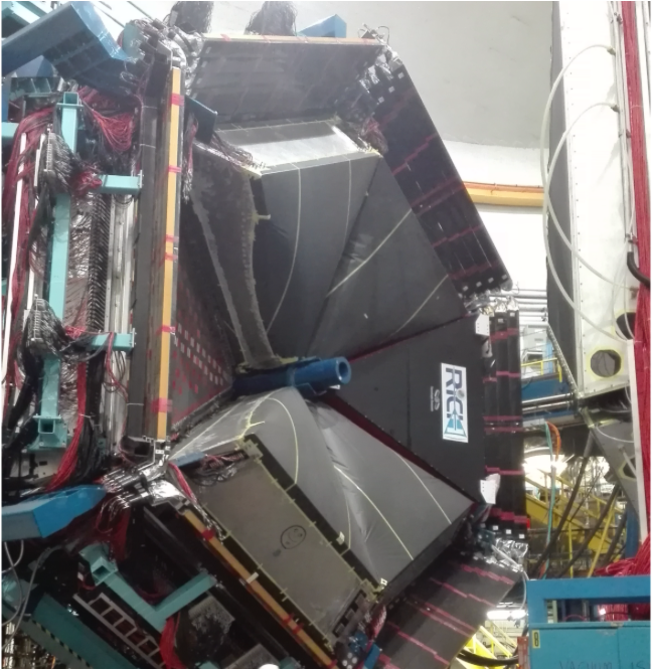
\includegraphics[width=0.80\columnwidth]{EPS/RICH_Installed.pdf}
\end{center}
\caption{The first module of the CLAS12 RICH installed in sector 4 of the Hall-B forward carriage}.
\label{Fig:RICHPic}
\end{figure}


In the CLAS12 kinematic regime, the expected production ratio of kaons to pions is about 1 to 10. Therefore, in order to 
keep the contamination of misidentified kaons at a few percent level, a pion to kaon rejection power of the order of 1:500 
is required.

The design of a RICH detector with these performances within the CLAS12 constraints was challenging, because of the peculiar 
trapezoidal shape and the stringent requirements in terms of material budget imposed by the downstream TOF and calorimeters 
detectors. Therefore, an effort was made in order to reduce the inactive material as much as possible. In addition, its large 
size (about 5 m$^2$ entrance window) imposed to reduce the area instrumented with photodetectors in order to contain the costs 
at an affordable level.

Simulation studies~\cite{RICH:first,RICH:ElAlaoui} and test of various prototypes with hadron beams~\cite{RICH:CERN} led to a non 
conventional proximity focusing geometry, incorporating an aerogel radiator, a system of planar and spherical mirrors and 
visible light photodetectors, in which the Cherenkov photons can be detected either directly or after reflections on the 
mirrors. A sketch of the detector is shown in Fig.~\ref{fig:RICHsketch}.

\begin{figure}
\begin{center}
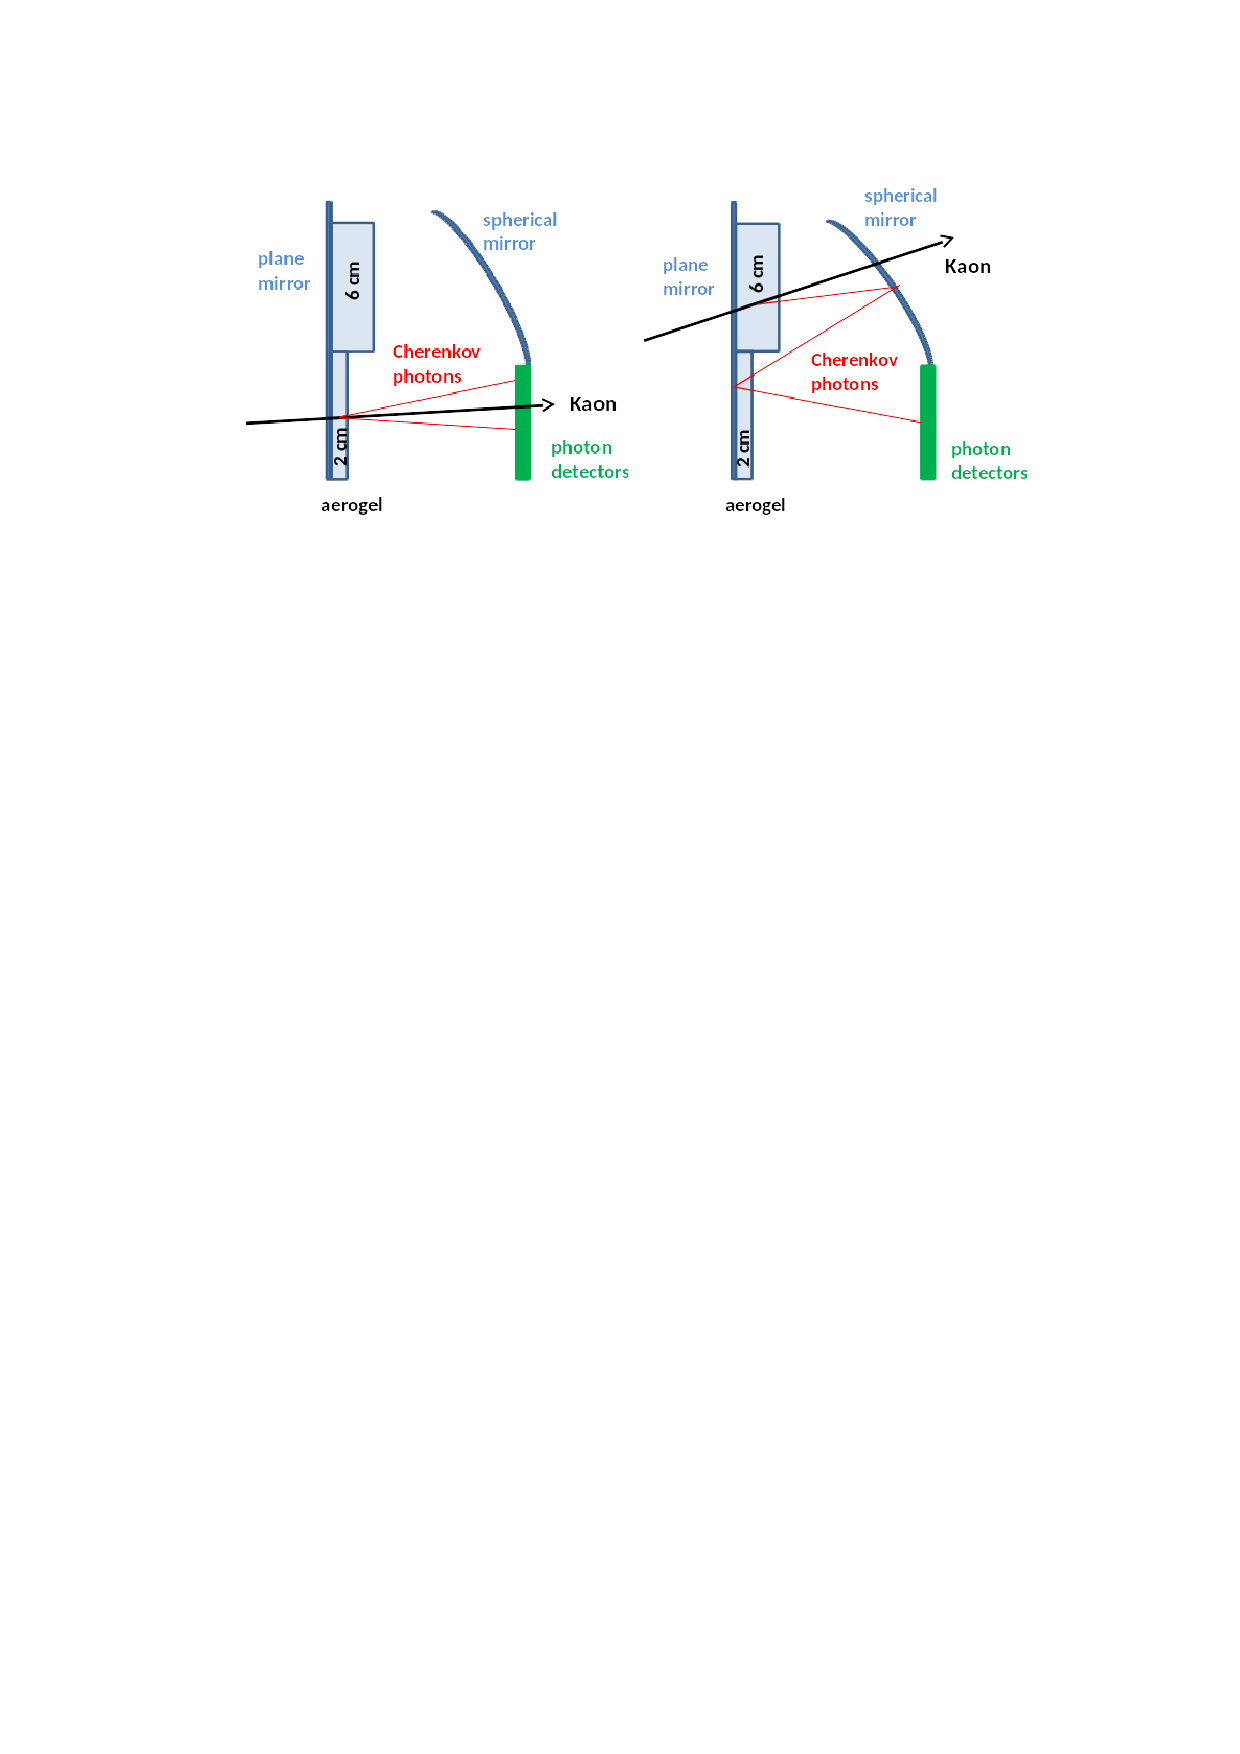
\includegraphics[width=0.50\textwidth]{EPS/Layout.pdf}
\caption{A schematic drawing of the CLAS12 RICH, whose hybrid optics design exploits direct 
imaging and light reflections to extend the angular and momentum coverage while limiting
the active area to only about 1 squared meter.}
\label{fig:RICHsketch}
\end{center}
\end{figure}

%-----------------------------------------------
\subsection{The Mechanical Structure}
%-----------------------------------------------

\begin{figure}
\begin{center}
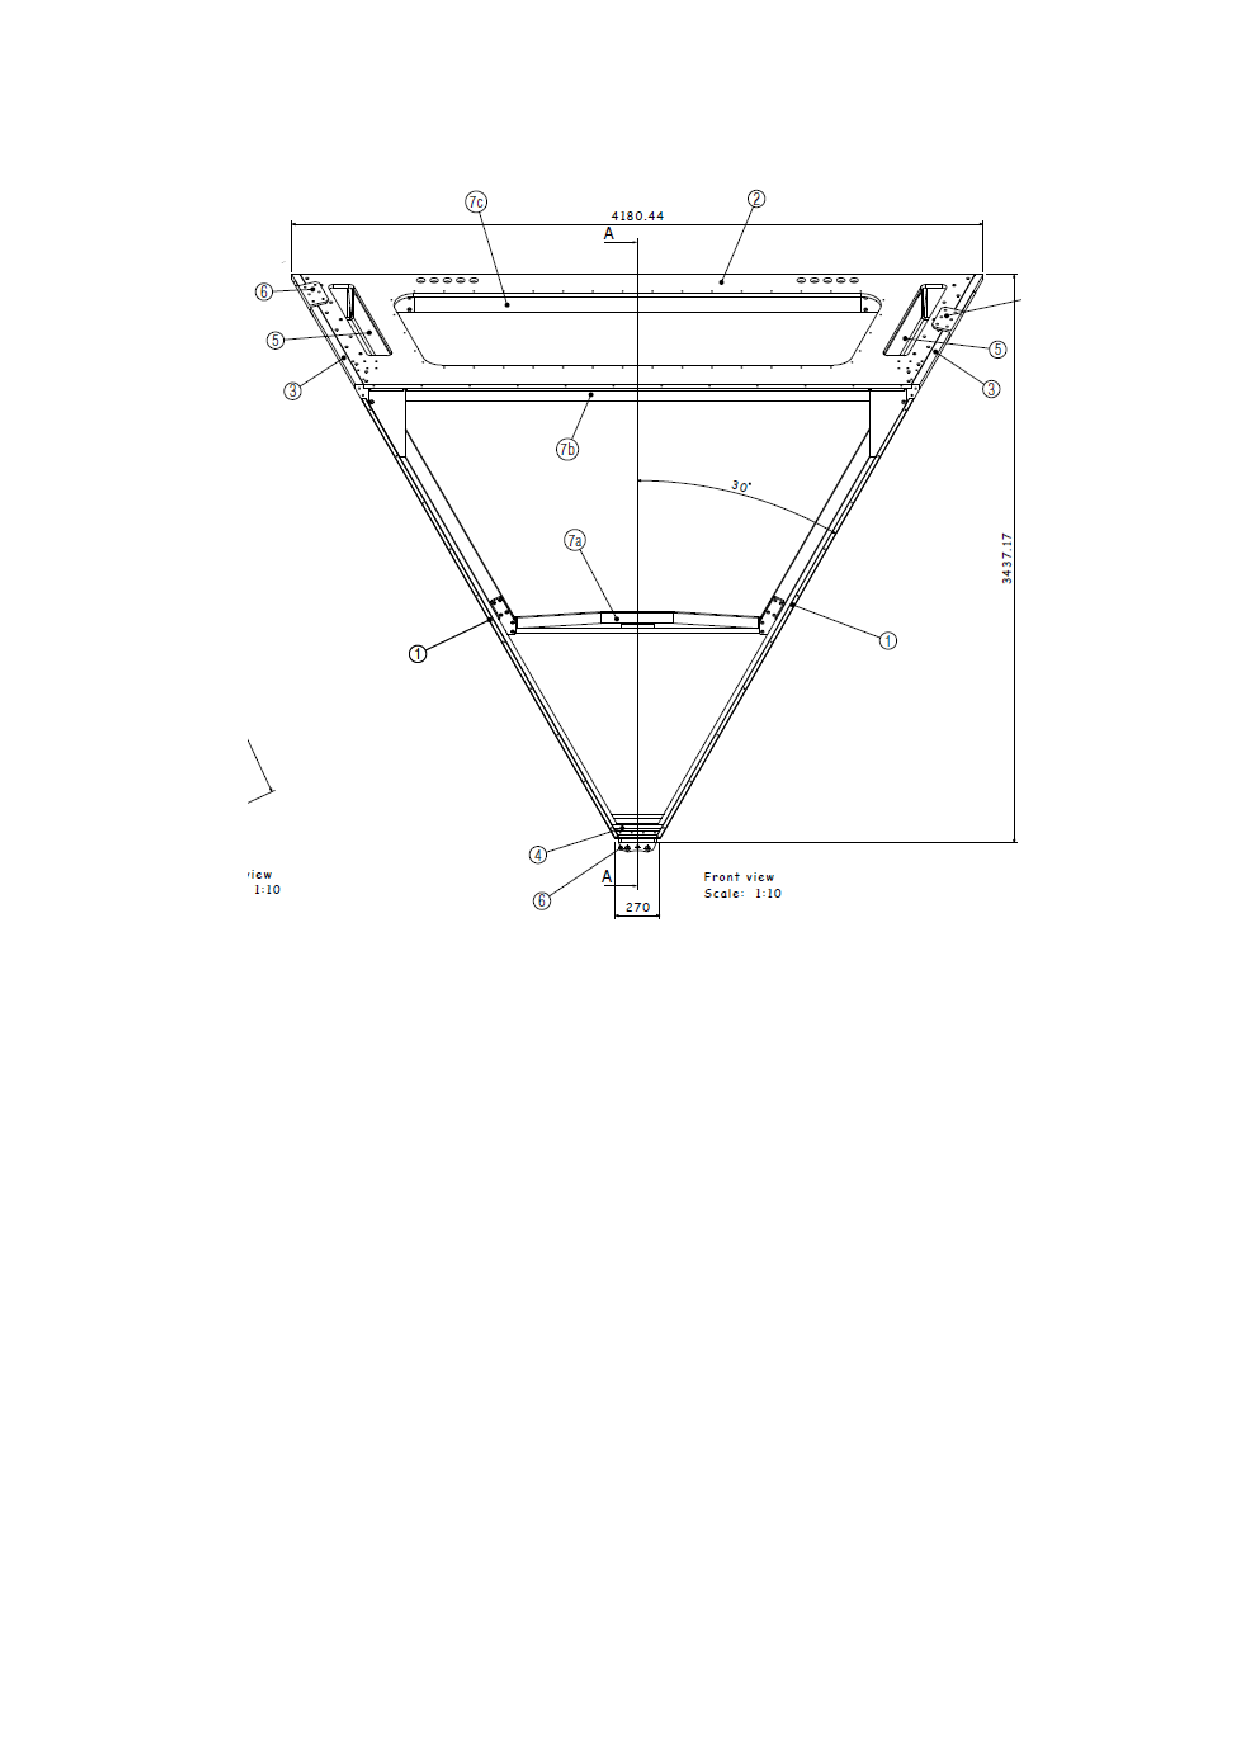
\includegraphics[width=0.40\textwidth]{EPS/Design_structure.pdf}
\caption{The composite frame of the RICH detecor. The components inside the CLAS12
acceptance (2, 7a, 7b, 7c) are made by carbon fiber.}
\label{fig:RICHframe}
\end{center}
\end{figure}

\begin{figure}
\begin{center}
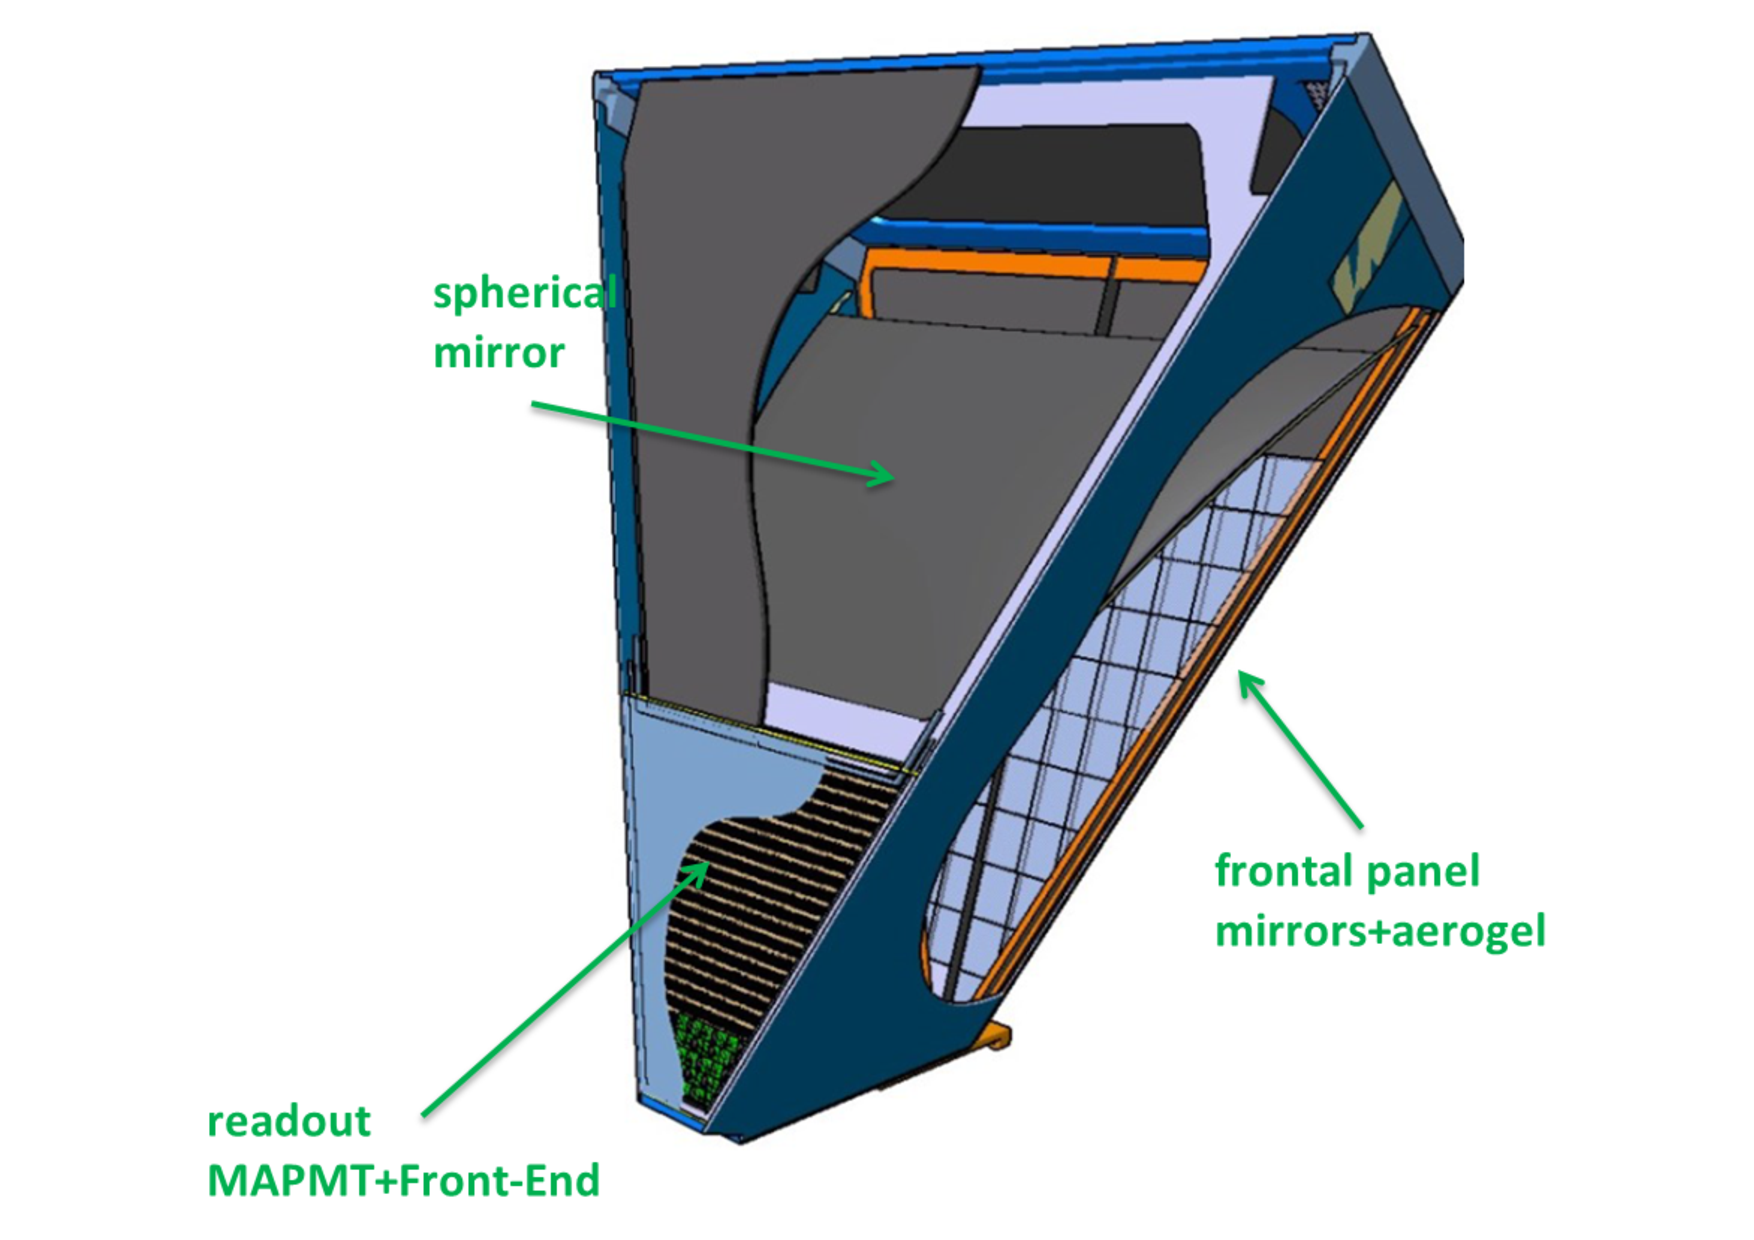
\includegraphics[width=0.45\textwidth]{EPS/RICH.pdf}
\caption{A schematic drawing of the CLAS12 RICH with the internal components highlighted.}
\label{fig:RICHexplo}
\end{center}
\end{figure}

The mechanical structure of the RICH, produced by the {\it Tecnologie Avanzate}~\cite{REF:Tecnavan} company, utilizes aluminum for 
the elements in the dead volume of CLAS12 and carbon fiber for the elements inside of the CLAS12 acceptance, see Fig.~\ref{fig:RICHframe}. 
For all the parts with large dimensions, the sandwich technique was used, in which two thin solid skins are glued together on a honeycomb core. 
The RICH mechanical structure was assembled on a frame especially designed to allow the installation of the internal components 
and of the closing panels, see Fig.~\ref{fig:RICHexplo}. 
Special attention was devoted to the structure rigidity to minimize stress and misalignments of the 
delicate optical components (mirrors and aerogel) during the assembly, transportation and installation.
For each of these phases, a dedicated FEM analysis was performed, see Fig.~\ref{}.

\begin{figure}
\begin{center}
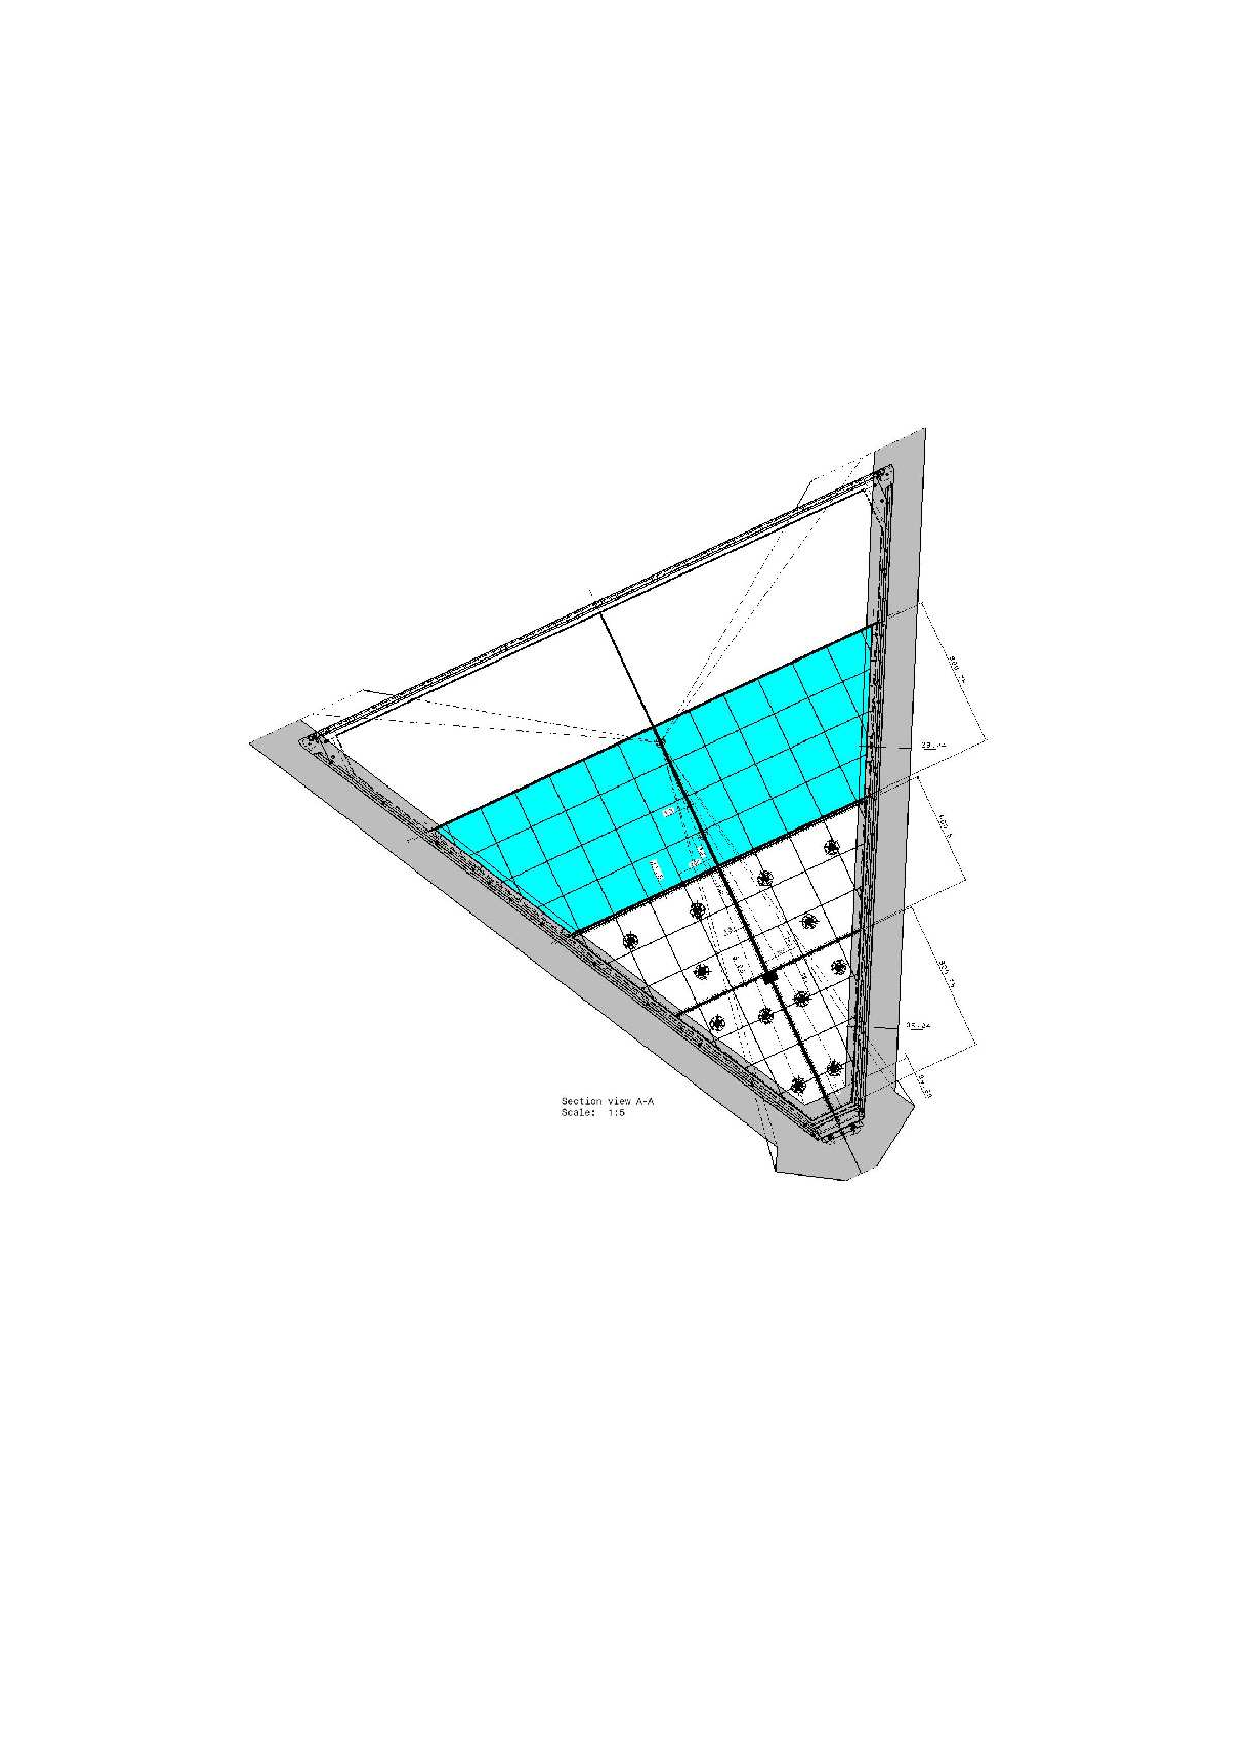
\includegraphics[width=0.40\textwidth]{EPS/Design_aerogel.pdf}
\caption{The aerogel tile configuration. The edge tiles have been shaped to match the RICH geometry. 
The 6 cm section (cyan) is made by two layers of 30 mm thick aerogel tiles installed on the front carbon fiber panel.
One layer of 20 mm tick aerogel tiles is mounted on the two front mirrors in the region close to the beam pipe. The 
aerogel is secured in place by a grid of nylon wires stretched on a 2 mm Aluminum perimetral frame.   
The mirror mounting points has been designed to stay outside the CLAS12 acceptance.}
\label{fig:RICHaero}
\end{center}
\end{figure}


%-----------------------------------------------
\subsection{The Aerogel Radiator}
%-----------------------------------------------

In the few GeV/c momentum range, the best radiator option is silica aerogel, which is being used by several particle and nuclear 
physics experiments worldwide~\cite{REF:Aerogel,REF:Belle}. The aerogel radiator used in the CLAS12 RICH is made by 102 large tiles 
with nominal refractive index $n=1.05$ produced by the {\it Budker and Boreskov Institute of Nuclear Physics} (Russia). In order to 
match the RICH geometry, the tiles were cut with squared $200 \times 200$ $\rm mm^2$ as well as pentagonal, trapezoidal and triangular shape,
see Fig.~\ref{fig:RICHaero}.  
The tiles are assembled in two separate sections. In the most forward section, the tiles have thickness of 20 mm and are installed on 
top of the frontal planar mirrors.  In the large angle sections, two layers of 30 mm thickness tiles are installed on the carbon fiber 
entrance panel of the RICH. Fig.~\ref{Fig:AeroB1} shows the 20 mm sections of the aerogel wall fully assembled.

A series of characterization measurements~\cite{RICH:RICH2016mc} was performed in order to determine the main optical and geometrical 
parameters of all the tiles. The results showed that all the tiles satisfied the required specifications. In particular, using the 
Hunt parametrization of the light transmission~\cite{Hunt}, the average values obtained over all the tiles are scattering length of 
$L_{scatt} = 50.5$ mm, transparency parameter $A_0 = 0.975$ and clarity parameter $C = 0.00512$ $\rm \mu m^4 / cm$. From these measurements, 
the expected photon yield for $\beta=1$ particles was computed and the tiles with highest yield were installed where the more demanding 
rejection power is expected.  

\begin{figure}
\begin{center}
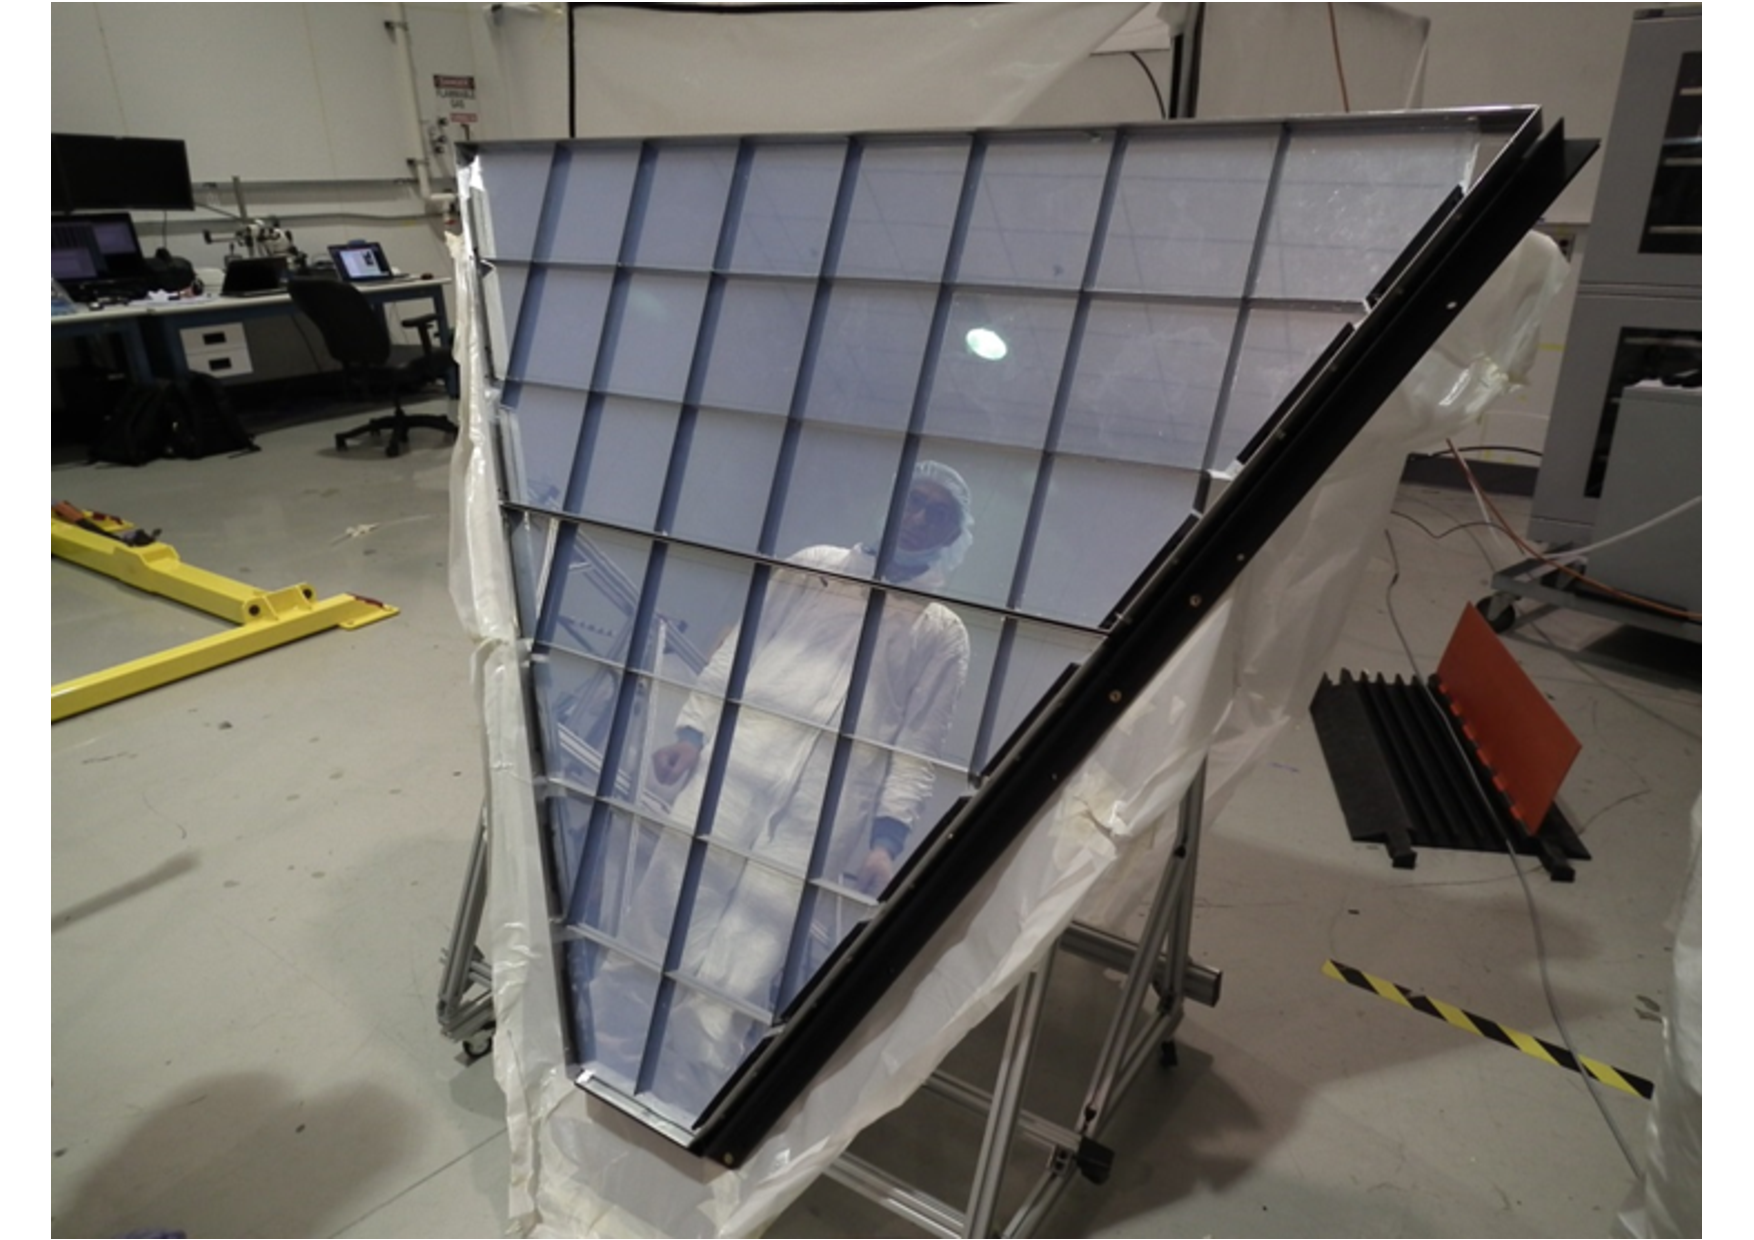
\includegraphics[width=0.35\textwidth]{EPS/aerogel_bottom.pdf}
\caption{The 20 mm thickness section of the aerogel.}
\label{Fig:AeroB1}
\end{center}
\end{figure}

\begin{figure}
\begin{center}
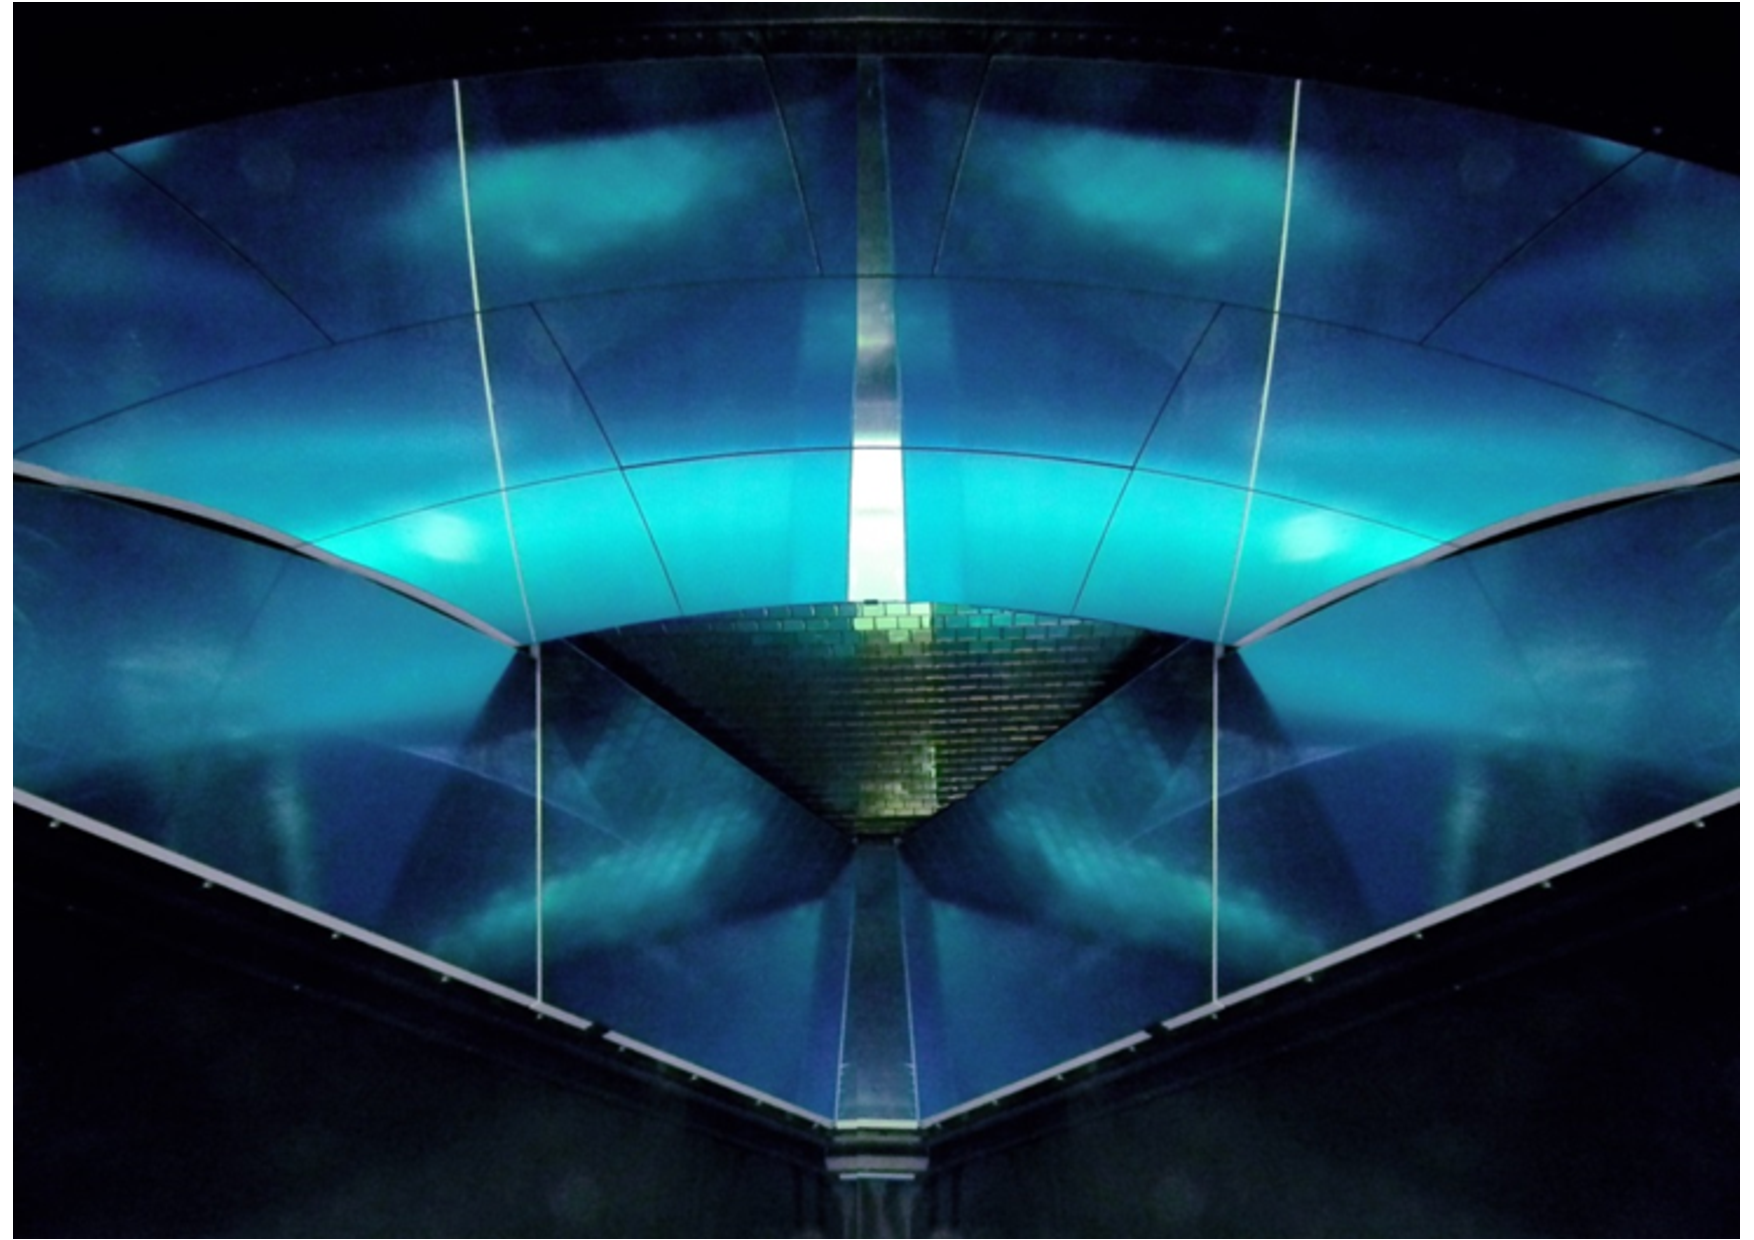
\includegraphics[width=0.4\textwidth]{EPS/mirrors.pdf}
\caption{The mirror system as it is seen from the RICH entrance panel.}
\label{fig:mirrors}
\end{center}
\end{figure}

%-----------------------------------------------
\subsection{The Mirror System}
%-----------------------------------------------

The mirror system is composed by 10 spherical mirrors, installed just before the exit panel of the RICH, and 7 planar mirrors installed 
on the entrance and lateral panels. The system was designed to minimize the photon loss and to direct as much as possible of the Cherenkov 
radiation toward the photodetectors. The mirror system as it is seen from the entrance panel is shown in Fig.~\ref{fig:mirrors}.

The spherical mirrors, produced by the {\it Composite Mirror Applications} company~\cite{REF:CMA}, are made by two layers of carbon fiber 
glued on a honeycomb core and were coated with the reflecting layer by the {\it Evaporated Coatings Inc}~\cite{REF:ECI}. The total area of 
these mirrors is about 3.5 m$^2$. The accuracy of the spherical surface was verified through the reflected spot size measurements, which 
also provides the average radius of curvature. All the mirrors exhibit a spot size smaller than 1.5 mm and a mirror-to-mirror variation in 
the radius below 0.5\%, well within the required specifications.

\begin{figure}
\begin{center}
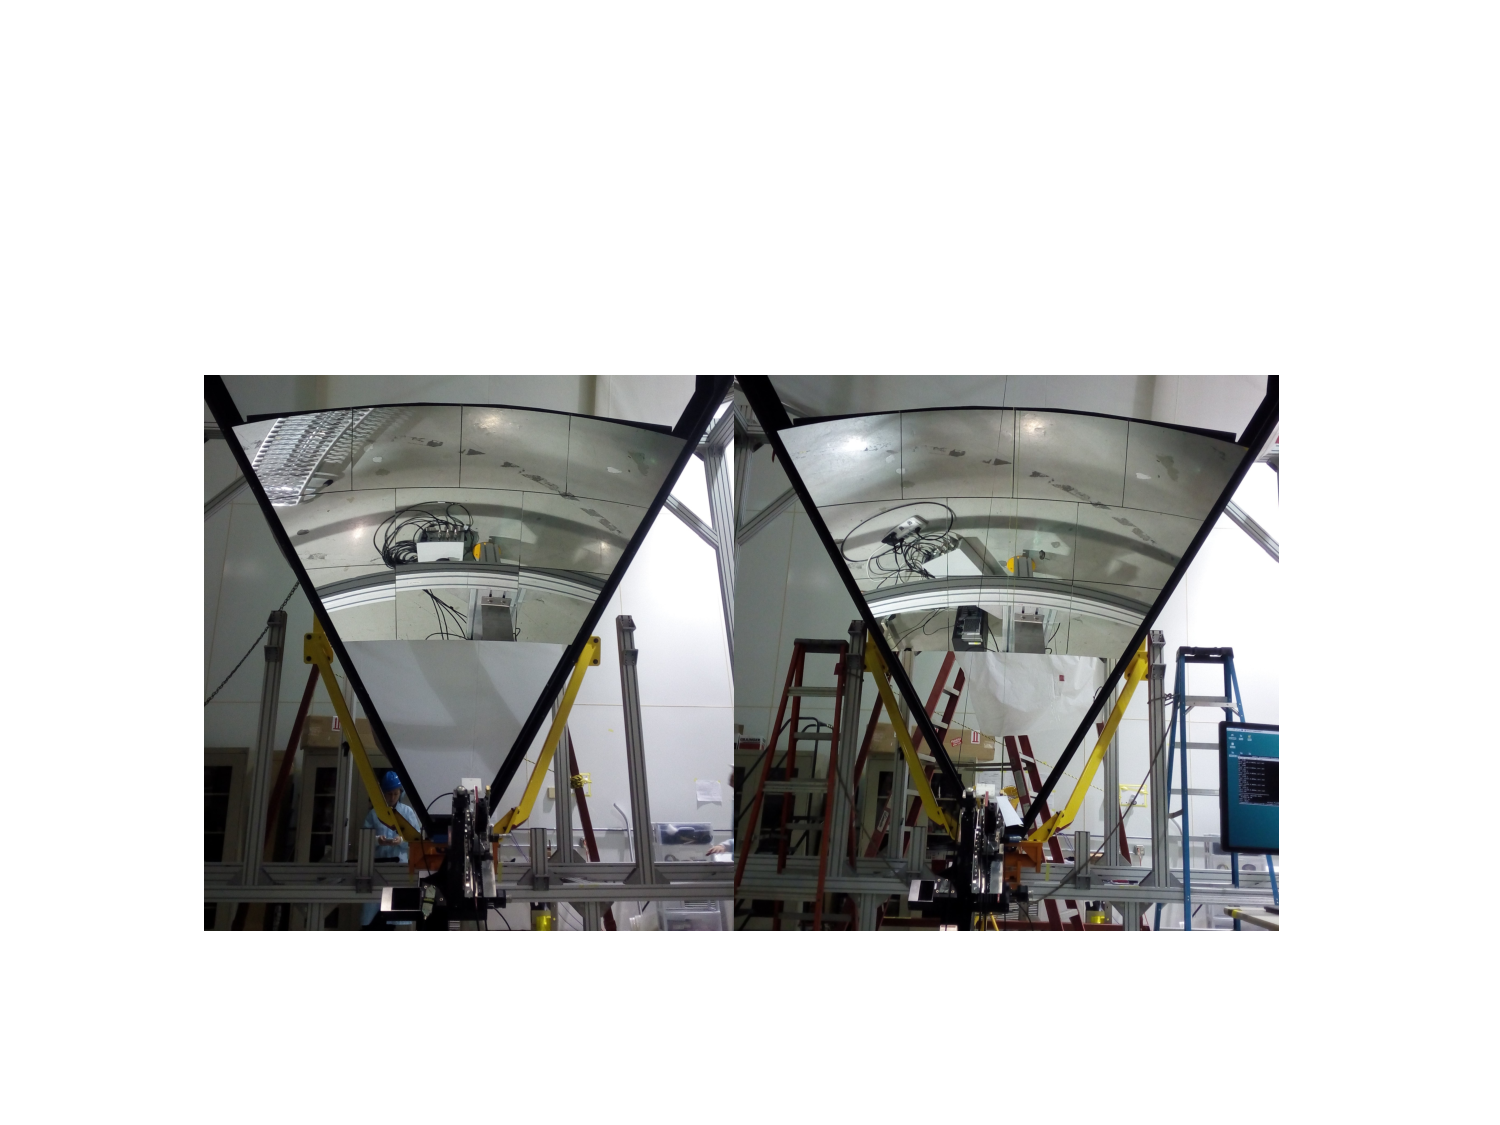
\includegraphics[width=0.44\textwidth]{EPS/Sphere_Align.pdf}
\caption{The spherical mirror before (left) and aftert (right) alignment.}
\label{fig:MirAlign}
\end{center}
\end{figure}

The planar mirrors, produced by the {\it Media Lario} company~\cite{REF:MediaLario}, are made by two thin layers of glass glued on a aluminum 
honeycomb core. Being in the acceptance of the detector, the frontal mirrors use very thin (0.7 mm) glass layers, while for the lateral ones 
thicker (1.6 mm) layers were used. This technology, used for the first time in nuclear physics experiments, allows to have mirrors with 
material budget comparable to the carbon fiber ones, but at much lower cost. The total area of the mirrors is about 6.5 m$^2$. The planarity 
of the mirror surface was measured by using a Coordinate Measuring Machine (CMM). Typically, the measured surface accuracy is of the order of few 
microns RMS, corresponding to a contribution to the angular resolution below 0.1 mrad, by far within the required specification of 0.3 mrad.

The characterization of both spherical and planar mirrors was completed by reflectivity measurements on several sample spots on the mirror 
surface in the range of wavelengths of interest from 350 to 600 nm. For all the mirrors, we obtained on average a reflectivity between 88\% 
and 90\%.

The planar mirror were aligned with respect the RICH structure with a precision of 0.1 mrad with the use of a CMM machine. The spherical
mirrors were aligned with a precision better than 0.1 mrad by converging the spot images of a pointlike source on the nominal center position, 
imaged by a XIMEA camera with a 1 cm wide CMOS sensor, see Fig.~\ref{fig:MirAlign}.


%-----------------------------------------------
\subsection{The Photon Detector}
%-----------------------------------------------
The goal of the CLAS12 RICH is to achieve a single photon-electron (SPE) Cherenkov angle resolution, dominated by the 
aerogel chromatic dispersion, of 4.5 mrad. 
At the RICH detector position, the CLAS12 torus fringe field is low enough to allow a flexible choice of the photosensor
technology, see Fig.~\ref{fig:MagFringe}.
%Early simulations~\cite{clas12:rich} led to a photosensor spatial resolution below 1~cm to fulfill the design value of 2~mrad angular resolution
%in the direct light configuration.
The flat panel Hamamatsu H8500 Multi-Anode PhotoMultiplier Tube (\MAPMT)~\cite{Ref:H8500} has been 
selected to achieve the design angular resolution, thanks to the enhanced sensitivity to the visible and near-UV light in conjunction with a matching geometrical 
layout of 64 pixels covering a 5x5 $\rm cm^2$ area with an excellent packing factor of 89\%.
Despite not advertised as the optimal choice in the SPE regime, such \MAPMT showed adequate performance 
in several laboratory tests~\cite{MAPMT:test} and at beam tests~\cite{RICH:CERN} when used in 
conjunction with an adapted readout electronics. Just after the RICH construction startup, the novel Hamamatsu 
H12700 became available, with the same layout of the H8500 but an optimized dynode structure for single 
photon detection~\cite{Ref:H12700}. 

The CLAS12 RICH is the first large-area detector to employ this type of multi-anode photo-multiplier. A total of 391
MAPMTs, corresponding to about 25000 pixels, are needed to cover the about 1 $\rm m^2$ trapezoidal active 
area of the first RICH module. 
The production of the RICH photon detectors (80 H8500 and 320 H12700) has been completed, achieving an
average gain of $2.7\cdot 10^6$, which corresponds to about 400 fC generated charge per SPE, see Fig.~\ref{fig:MAPMTGain}.

\begin{figure}[t]
\begin{center}
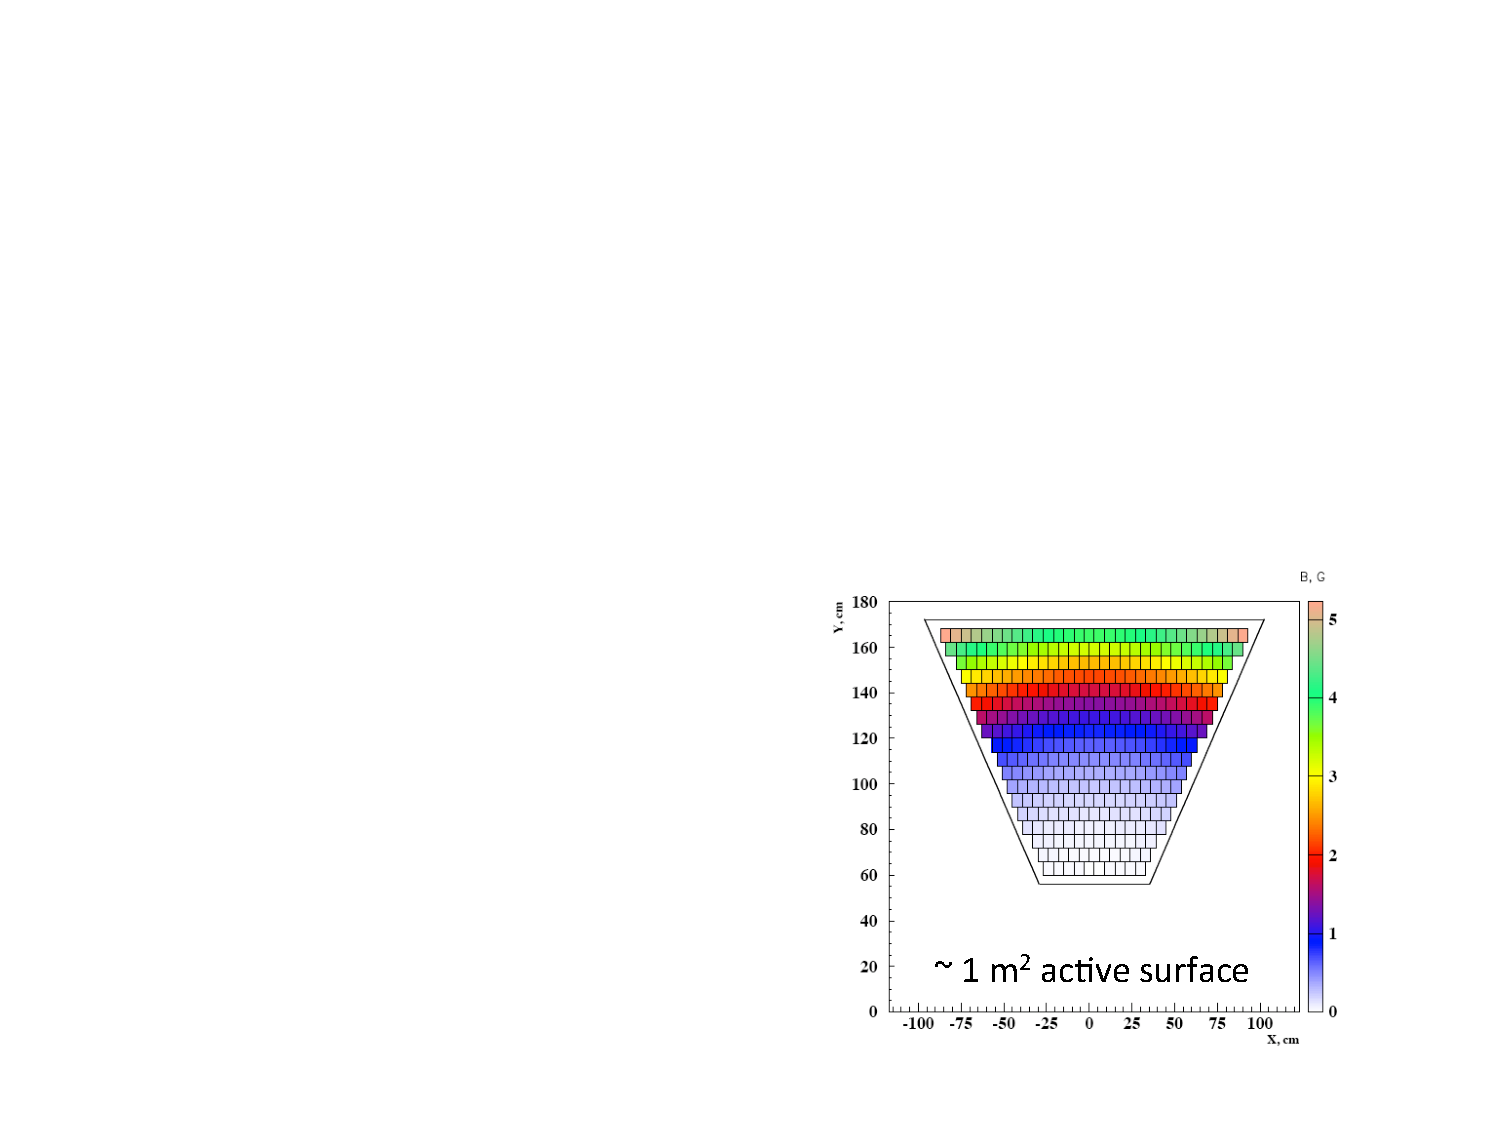
\includegraphics[width=0.65\columnwidth]{EPS/Field.pdf}
\end{center}
\caption{The RICH photon detector area with the simulated torus frienge field strength.}
\label{fig:MagFringe}
\end{figure}

\begin{figure}[t]
\begin{center}
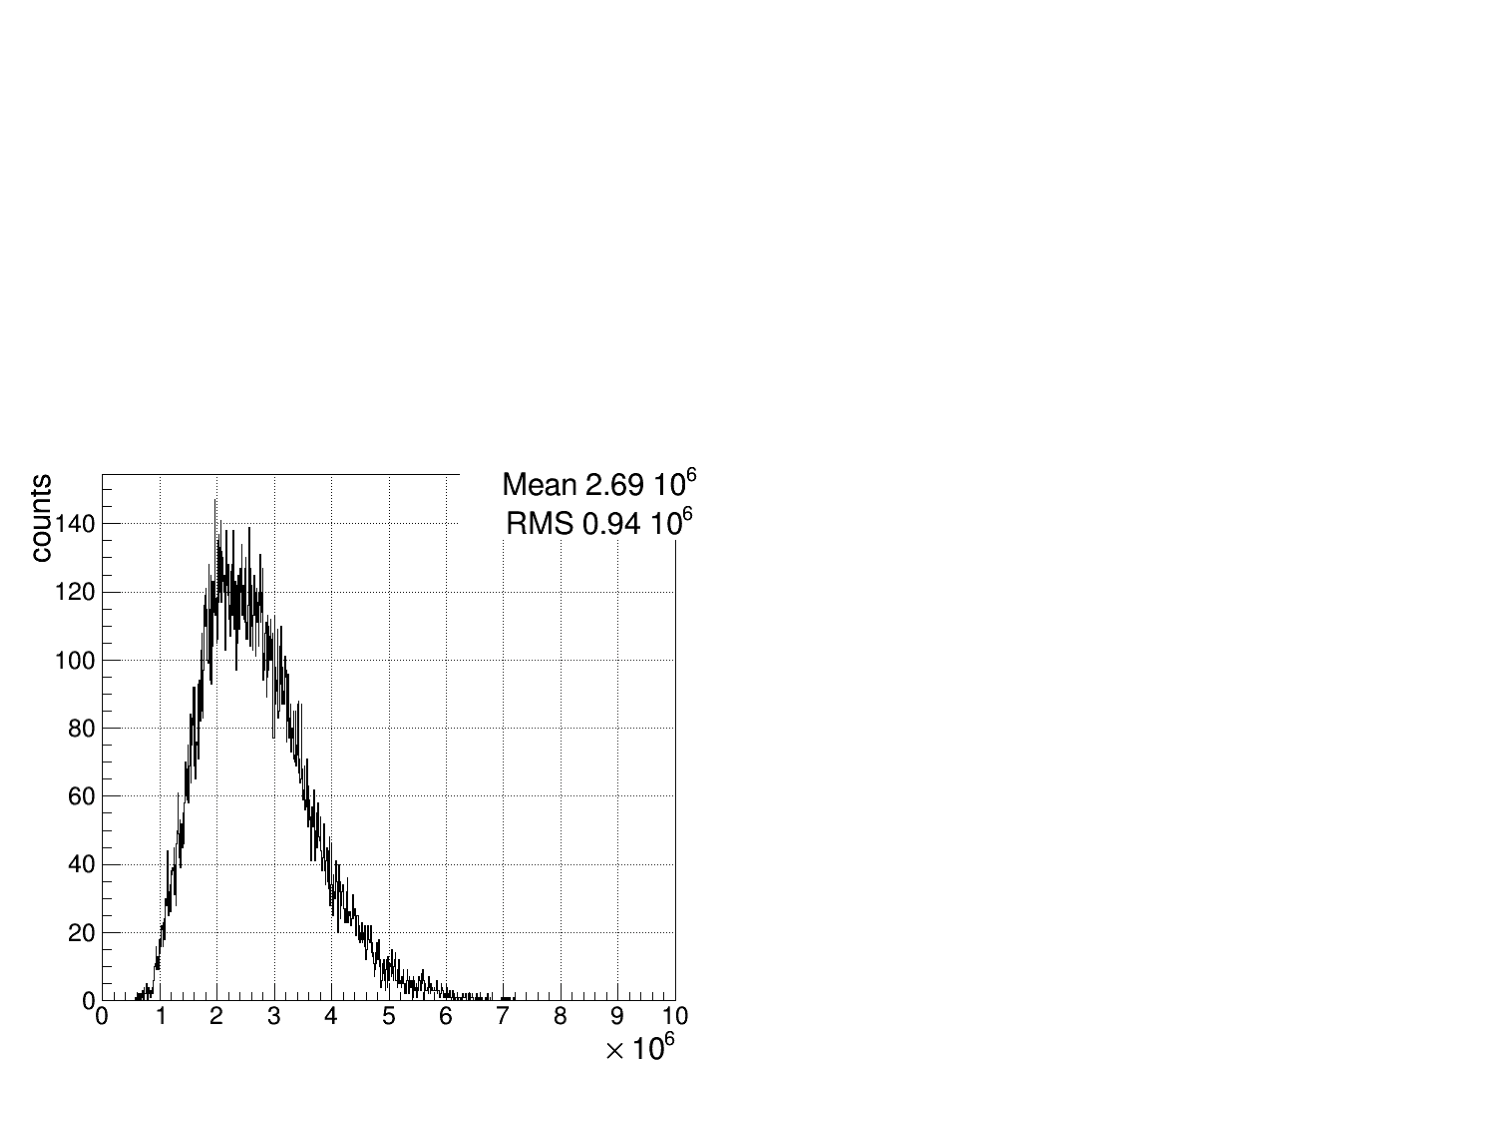
\includegraphics[width=0.65\columnwidth]{EPS/Gain.pdf}
\end{center}
\caption{Distribution of the data-sheet gains of the 25000 RICH MAPMT channels.}
\label{fig:MAPMTGain}
\end{figure}

%-----------------------------------------------
\subsection{The Readout Electronics}
%-----------------------------------------------

\begin{figure}[t]
\begin{center}
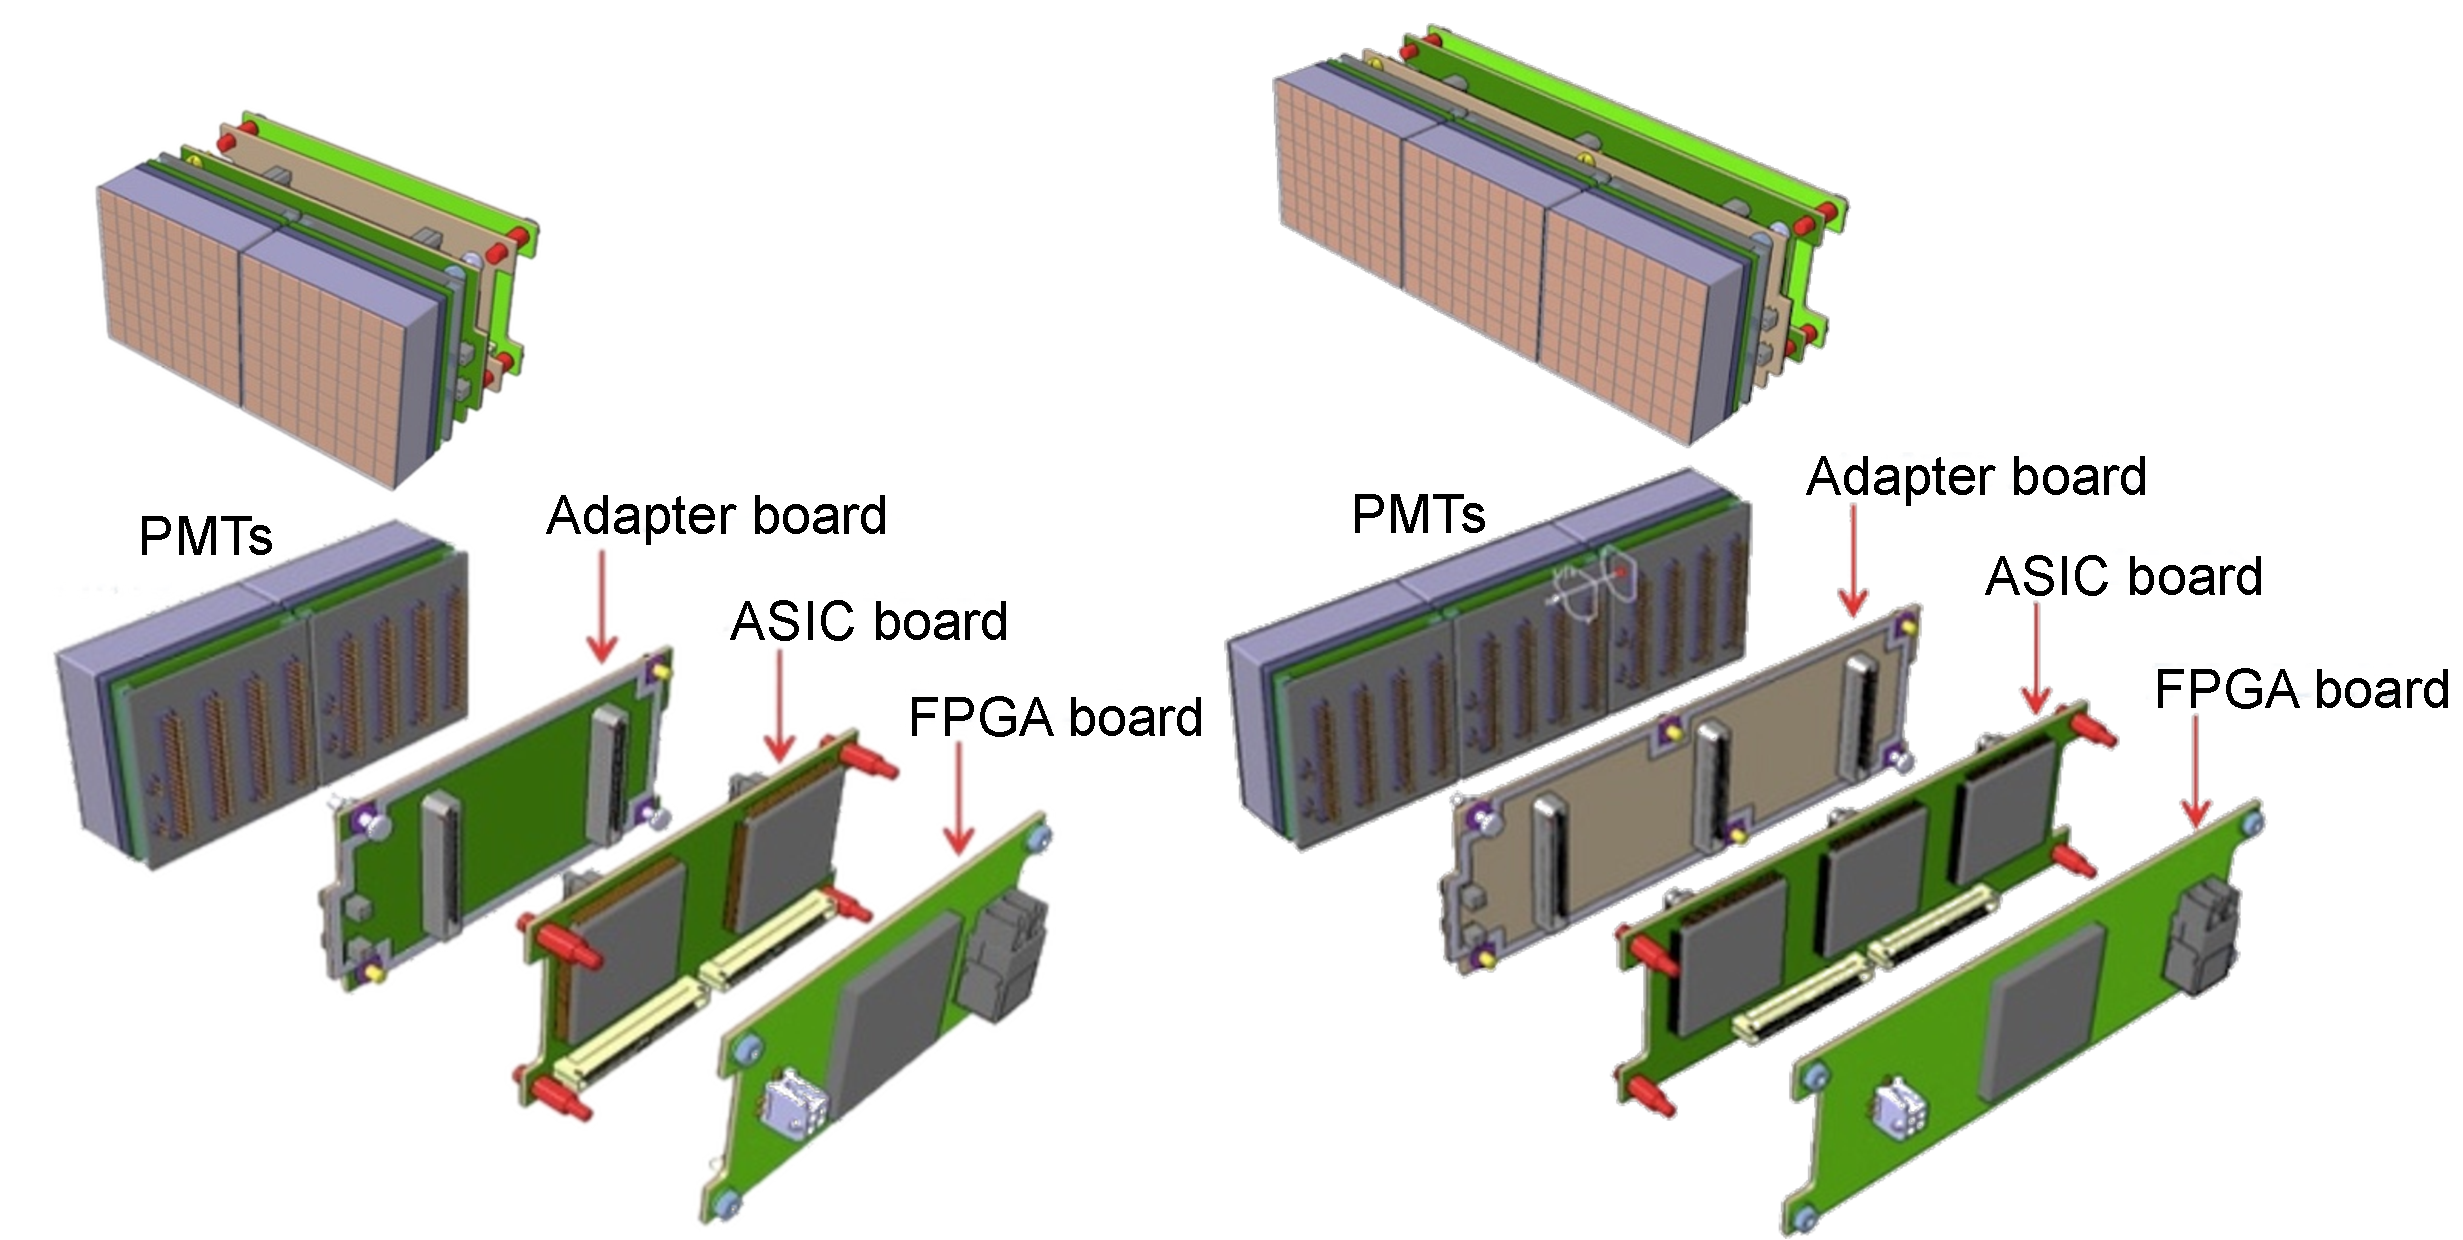
\includegraphics[width=1.00\columnwidth]{EPS/TileAssembly.pdf}
\end{center}
\caption{The CLAS12 RICH readout unit design (see text for details).}
\label{fig:EleTile}
\end{figure}

\begin{figure}[t]
\begin{center}
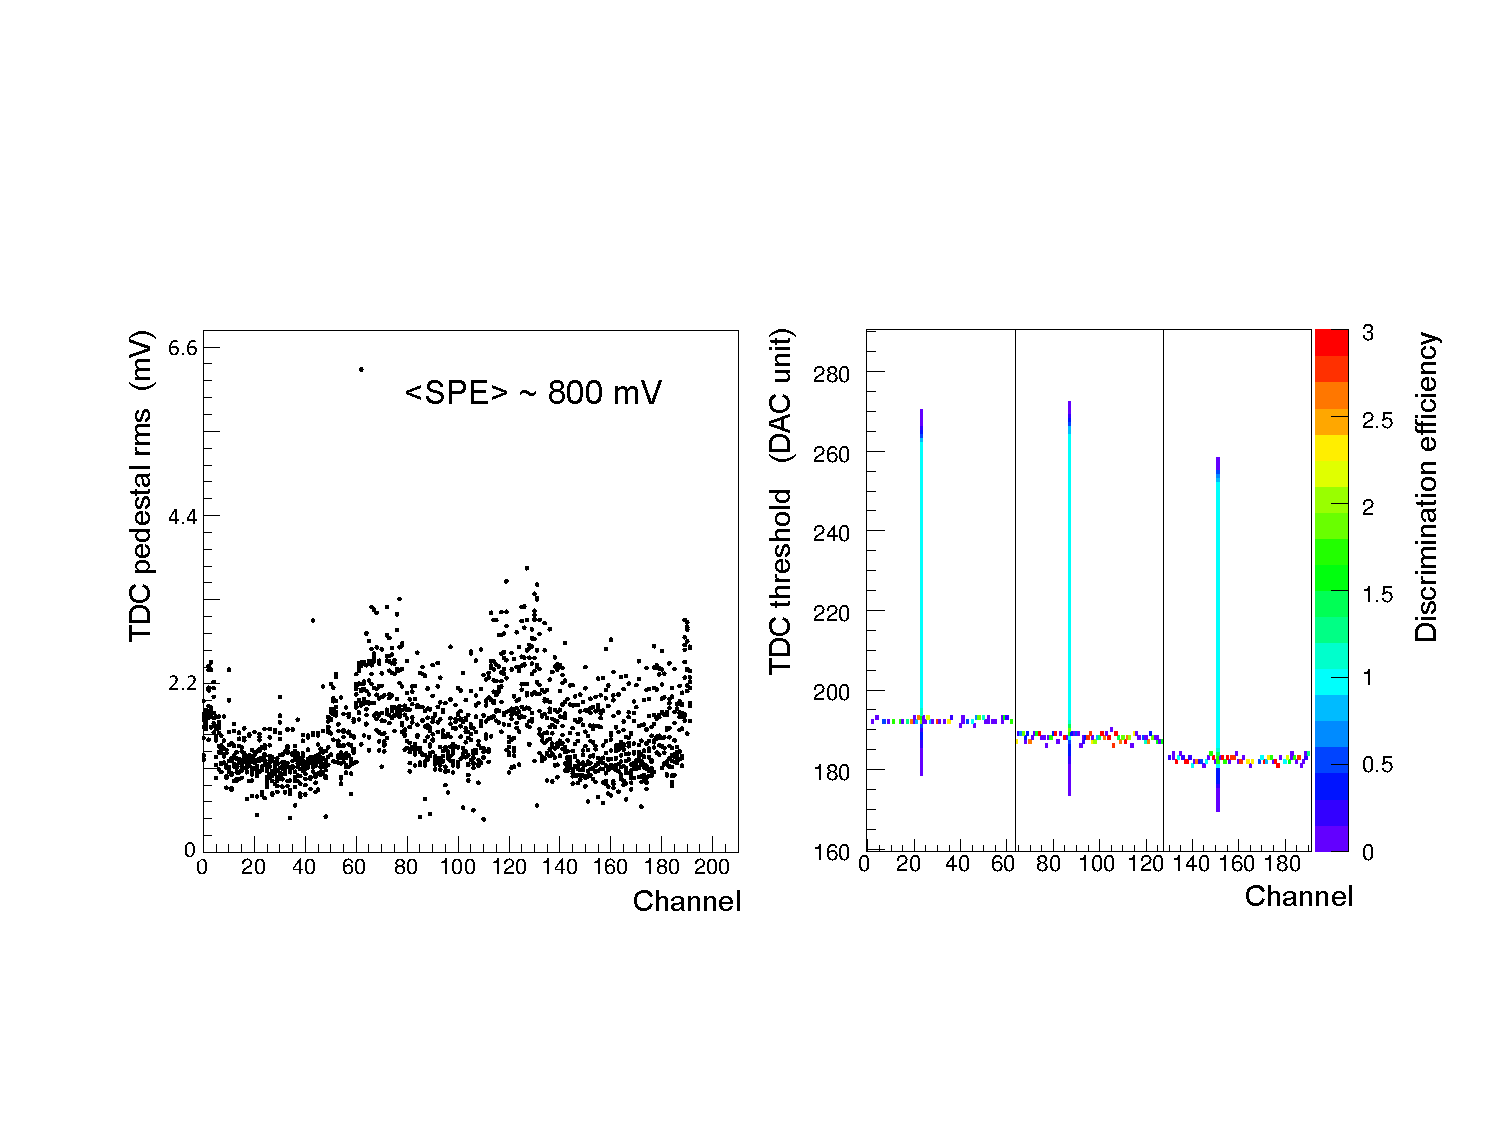
\includegraphics[width=1.0\columnwidth]{EPS/Figure2.pdf}
\end{center}
\caption{(Left) Pedestal RMS, as measured on a test point, of the 192 channels of
the $3\times$ MAROC boards
during the production quality assurance. The measured RMS values are below 4 mV while
the single photo-electron signal is expected around 800 mV. (Right) Logic discrimination efficiency
as a function of the MAROC channel, for a range of programmed thresholds. A test pulse
corresponding to 60 fC, i.e. about 1/7 of the expected typical single photo-electron discharge,
is generated by the programmable on-board pulse generator and injected in channel 23 of each chip.
Close to the pedestal value, spurious fluctuations are discriminated in all channels (efficiency
greater than 1). At threshold values below the pedestal, the system digitized the undershoot of the
bipolar shaped signal.}
\label{Fig:pedquality}
\end{figure}

\begin{figure}[t]
\begin{center}
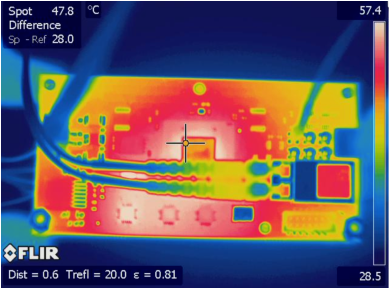
\includegraphics[width=0.70\columnwidth]{EPS/FPGA_heat.pdf}
\end{center}
\caption{The CLAS12 RICH readout unit design (see text for details).}
\label{Fig:EleTile}
\end{figure}

The RICH front-end electronics is designed to ensure 100\% efficiency at 1/3 of the average photo-electron signal level, 1 to 4 
gain spread compensation, time resolution of the order of 1 ns to distinguish direct from reflected photon hits, 
and a trigger rate up to 20 kHz and 8 $\rm \mu s$ trigger latency. 

The front-end electronics is organized in compact units (tiles) mechanically designed to fit the MAPMT dimensions,
each serving two or three MAPMTs, thus allowing the tessellation of large surfaces with minimum dead space 
and material budget, see Fig.~\ref{fig:EleTile}. Each readout unit comprises three boards with complementary 
functions.

A feed-through {\it adapter board} provides the electrical connectivity of the sensors with the external readout 
system while preserving the adequate light and gas tightness of the inner detector volume when mounted on the 
RICH carbon fiber supporting panel. It also distributes the sensor bias voltage (with -1000~Volts as
nominal value). The {\it signal processing board} is based on the MAROC3 
chip~\cite{MAROC3:chip}, a 64-channel microcircuit dedicated to MAPMT pulse processing. Each channel comprises
a low impedance adjustable gain preamplifier followed by two highly configurable shaping sections with independent processing. 
The first section embeds a slow shaper and a sample and hold structure to allow linear charge measurements up to 5 pC.
Requiring short trigger delays and multiplexed access, this feature is used as a RICH calibration tool.  
The second section features a fast shaper and an adjustable threshold discriminator to produce, for each input signal, a 
start and stop logic pulse.
These are stored in a 8 $\rm \mu s$ deep circular memory allowing a parallel, almost 
dead-time free, readout. The fast shaper works in an almost saturated regime to maximize the discrimination efficiency. 
%The MAROC chip is configured and read out by a {\it FPGA board} optically linked with the data acquisition back-end (DAQ) made by 
%sub-system processor (SSP) modules inside a VSX/VME crate.  
The MAROC chip is configured and read out by a {\it FPGA board} optically linked to the data acquisition back-end (DAQ) 
using the JLab Sub-System Processor (SSP), which resides in a VXS/VME crate.
The current firmware version includes a 1 ns precision timestamping of the logic pulses.

%FPGA = Field Programmable Gate Array

A constant-threshold binary readout requires a good stability of the baseline (pedestal) and definition of the
working point (gain and threshold). Their programmed levels are here expressed as Digital-to-Analog Converter (DAC) units. 
During the board production, quality assurance tests confirmed the excellent sensitivity 
of the logical readout, able to discriminate signals down to a few percent of a single photon-electron discharge,
see Fig.~\ref{Fig:pedquality}.


%-----------------------------------------------
\subsubsection{Characterization}
%-----------------------------------------------

\begin{figure}[t]
\begin{center}
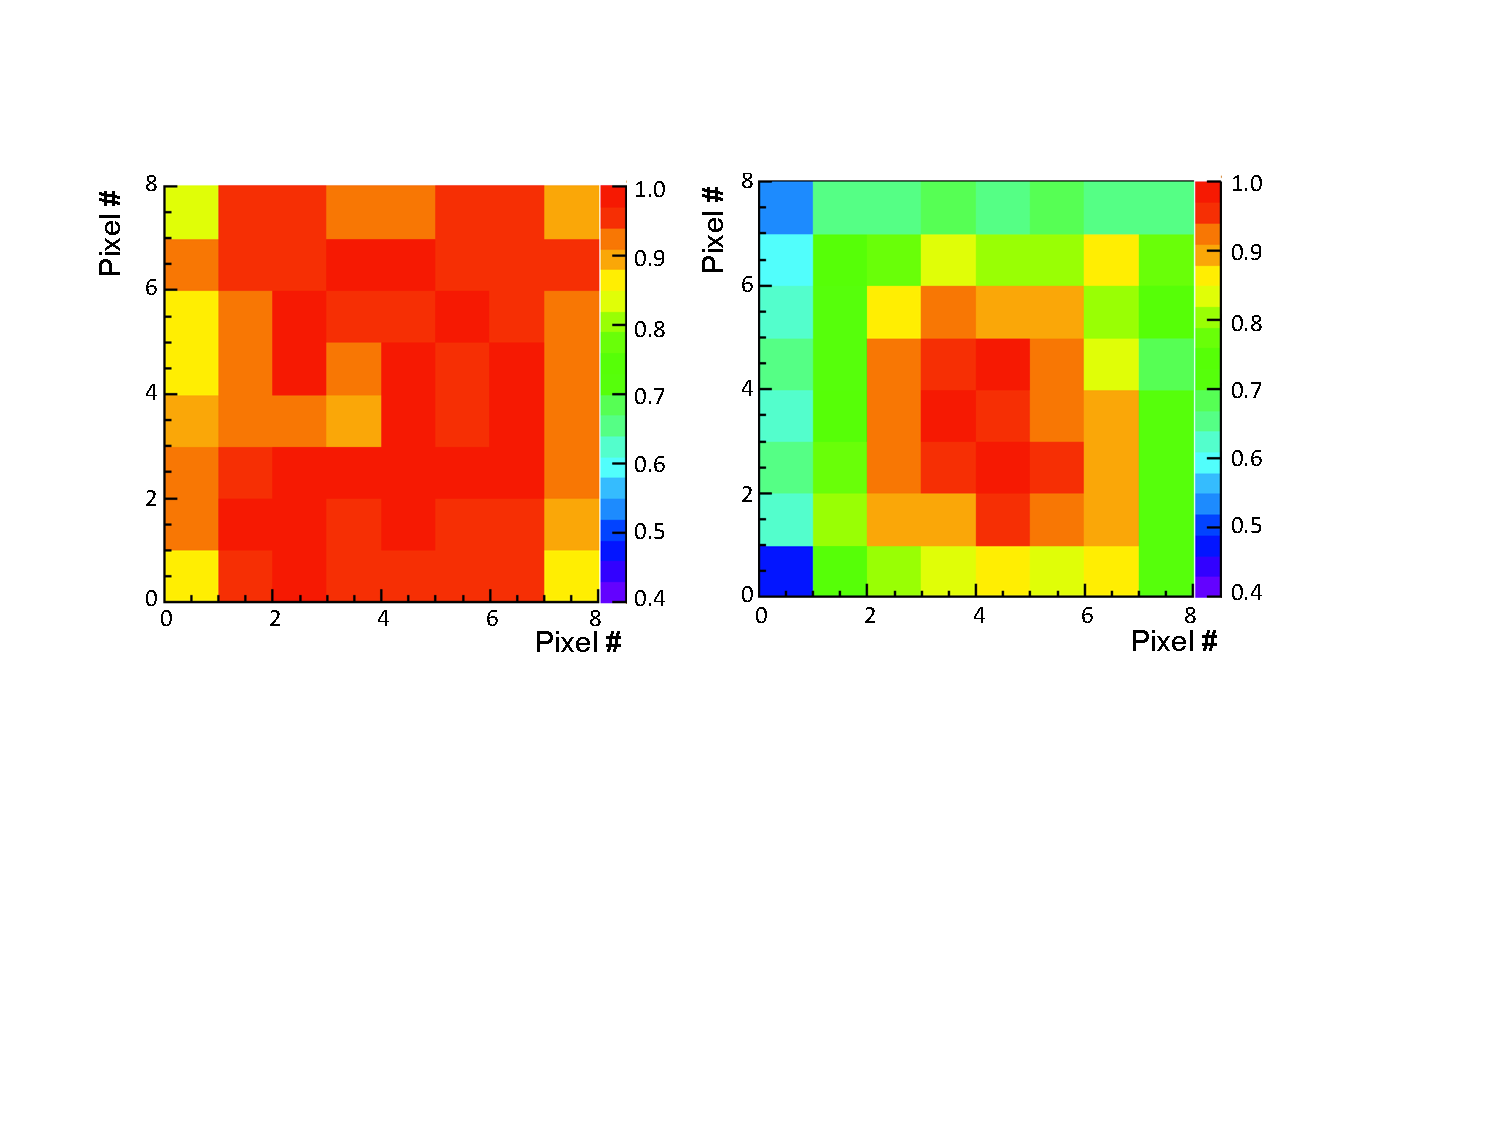
\includegraphics[width=1.0\columnwidth]{EPS/Figure3.pdf}
\end{center}
\caption{(Left) Example of MAPMT efficiency map normalized to the maximum pixel efficiency.
Data show an almost flat behavior at values close to 1 except for the edge pixels.
(Right) Example of MAPMT gain map normalized to the maximum pixel gain. The visible 1:2
variation is expected for this type of sensors and can be compensated by the electronics.}
\label{Fig:EfMap}
\end{figure}

\begin{figure}[t]
\begin{center}
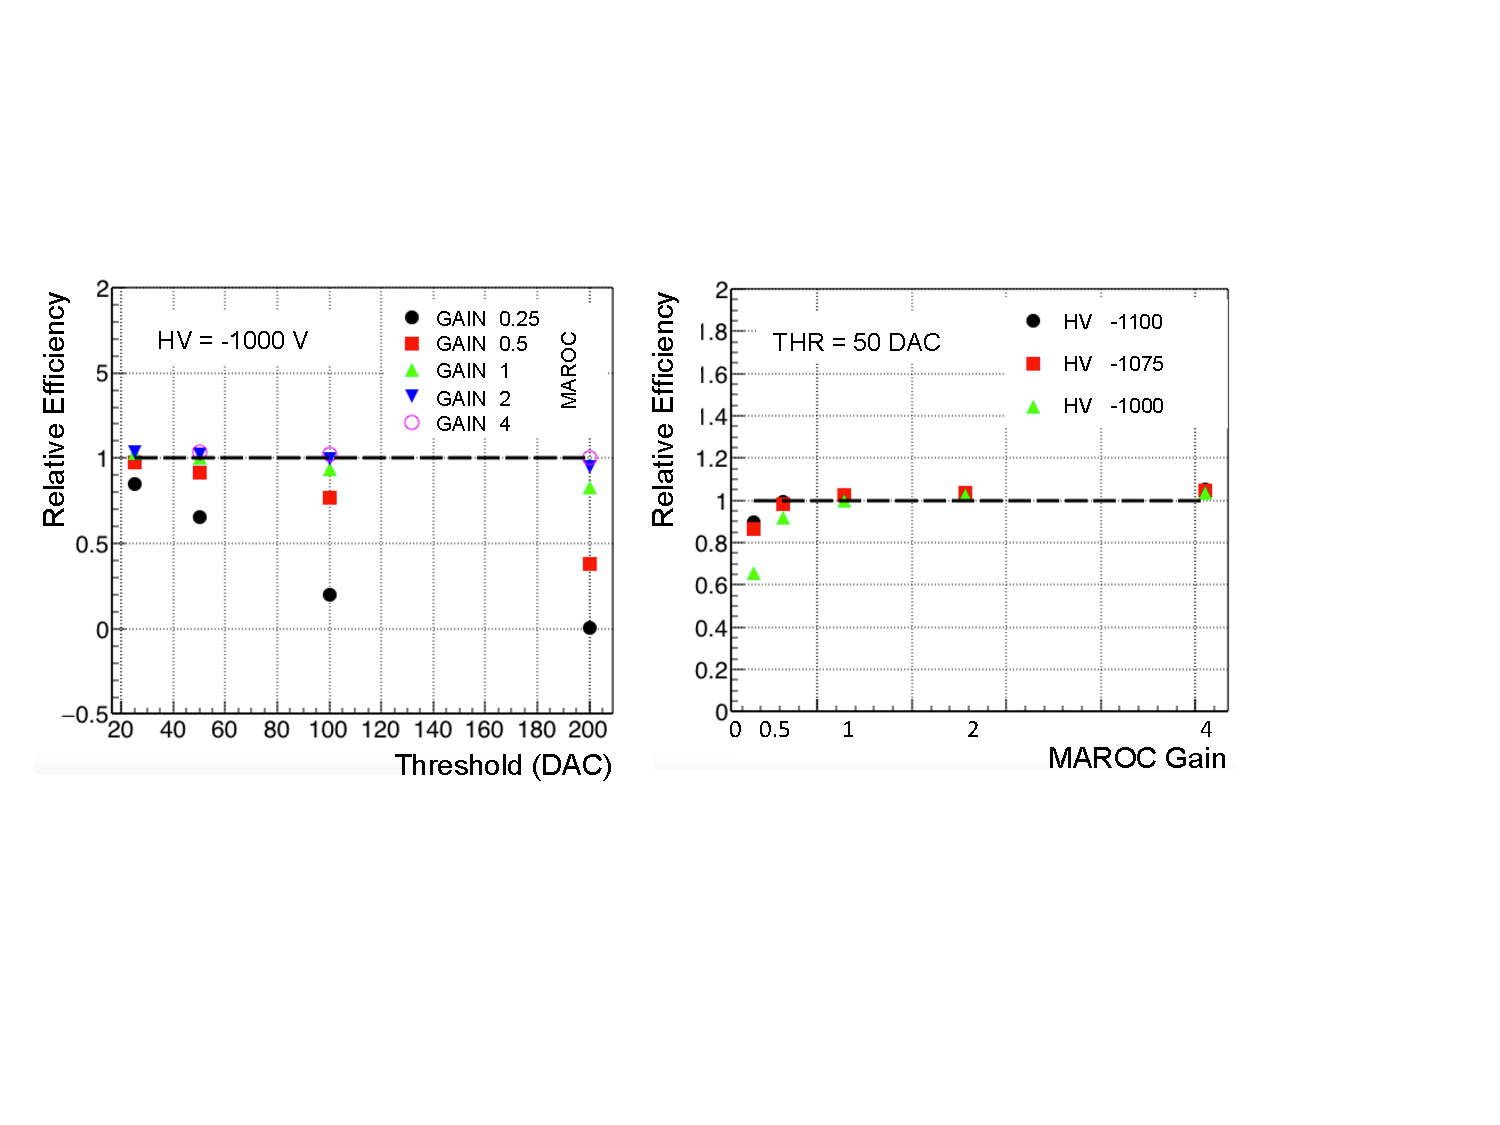
\includegraphics[width=1.0\columnwidth]{EPS/Figure4.pdf}
\end{center}
\caption{Relative SPE detection efficiency as a function of the working parameters: bias voltage,
MAROC preamplification gain and discriminator threshold. The plots show the dependence on two
parameters while keeping fixed the third: bias voltage (left) or threshold (right).
Data are normalized to the reference point at HV=-1000~V, gain=1 and threshold=+50 DAC. Values
greater than 1 are likely due to the cross-talk contribution.}
\label{Fig:EfScan}
\end{figure}

Each readout unit was characterized in laboratory tests using a pico-second precision pulsed PicoQuant laser of 
405 nm wavelength. A light diffuser was used in order to uniformly illuminate the whole sensitive area and integrate all
the local variations of the sensor response. The laser pulse intensity was tuned and optical neutral density filters added 
in order to deliver on average 3 photon hits per MAPMT. The recorded single-photon spectra allowed
to map the relative gain and efficiency of the 64 pixels of each MAPMT~\cite{MAPMT:laser}, see Fig.~\ref{Fig:EfMap}. 
%The two device types have been extensively studied with a picosecond pulsed laser beam in the SPE 
%regime~\cite{MAPMT:laser}, showing 
All the MAPMTs were fully tested 
and characterization parameters were extracted by fitting a detailed model of the SPE spectrum,
developed at JLab~\cite{MAPMT:model}.
Data showed that the H12700 has, on average, a 10\% better efficiency than the H8500, 
likely due to the improved photocathode performance. 
The recorded information
can be useful for the likelihood definition of each particle hypothesis in the RICH reconstruction. 
In addition, the SPE spectra allow to study the efficiency dependence on the working parameters, i.e. MAPMT bias voltage, 
MAROC pre-amplification gain and threshold. Data indicated the efficiency reaches a plateau over a wide range of 
working parameter values, see Fig.~\ref{Fig:EfScan}. The plateau would correspond to the region where all the MAPMT discharges 
are digitized and the efficiency ultimately depends on the quality of the photocathode. The plateau is a consequence
of the saturated mode employed in the MAROC binary readout and allows a flexible definition of the working point,
a crucial feature when dealing with a large number of channels in the challenging single-photon regime.

%Several tests have been performed with cosmic rays at various stages of the detector assembling. In the absence of a precise
%measure of the cosmic particle momentum it was not possible to perform a study of the Cherenkov angle resolution.
%Nevertheless, cosmic runs allowed to validate the translation tables relating electronic channels with pixel positions, 
%develop the ring reconstruction software, verify the stability of the system, and test the performance of the services 
%(power supplies, cooling, readout, slow-control, interlock). 

%With the full detector assembled, the measured pedestal RMS was initially at the level of few DAC units. 
%In order to properly refer to the same ground the whole composite readout system, powered by 156 floating 5V low-voltage lines, 
%a grounding grid was realized connecting all the boards with the detector chassis. With the grid, 
%%to the same ground the whole composite readout system powered by a 5~V floating low-voltage, 
%the typical pedestal RMS was reduced to 
%values comparable with the ones measured in the quality assurance tests and at the limit of the readout sensitivity, 
%i.e. at the level of 1 DAC and thus negligible, see Fig.~\ref{Fig:GroundG}.

%-----------------------------------------------
\subsection{Services}
%-----------------------------------------------


%-----------------------------------------------
\section{Assembly and preliminary tests}
%-----------------------------------------------

The RICH vessel was mounted on a large Aluminum frame allowing rotations from the vertical to the horizontal position,
as required by the various assembling phases.
Each inner element was installed on the mechanical structure after the completion of the characterization
tests. This assembly phase included also a detailed survey of the position and alignment
of each inner element, in particular the mirrors, with respect to the mechanical structure of the detector.
The lateral mirrors were the first elements installed followed by the spherical mirror.


The RICH readout system, composed by 138 tiles with 391 MAPMTs for a total of 25024 independent channels, was assembled on a 
dedicated carbon fiber panel. An independent Aluminum support was employed to get easy access and allow rotations during the 
functionality tests. 
The MAPMTs plane is shown in Fig.~\ref{fig:mapmts},
while the fully assembled Front End electronics is shown in Fig.~\ref{fig:electronics}.
The complete readout system was eventually moved into the the RICH and the closing panels temporarely mounted 
on the detector to test of the light and gas thightness of the system, prior of aerogel installation.

The aerogel was the last element installed, being the most sensitive to the external conditions. Each tile
were inspected and mounted in a pre-selected location of the supporting element, being the latter a carbon fiber panel 
(6 cm layer) or a front mirror with the Al frame (2 cm layer). The location was defined depending on the
aerogel tile shape and optical quality to maximize the overall performance. During assembling, the aerogel panels were 
maintained in a low humidity atmosphere (around 20 \%
relative humidity) to prevent moisture absorption. When ready, they were all mounted at once onto the RICH to allow an
instantaneous start of the nitrogen conditioning of the inner RICH volume and minimize the exposure to 
the external weather conditions.

\begin{figure}
\begin{center}
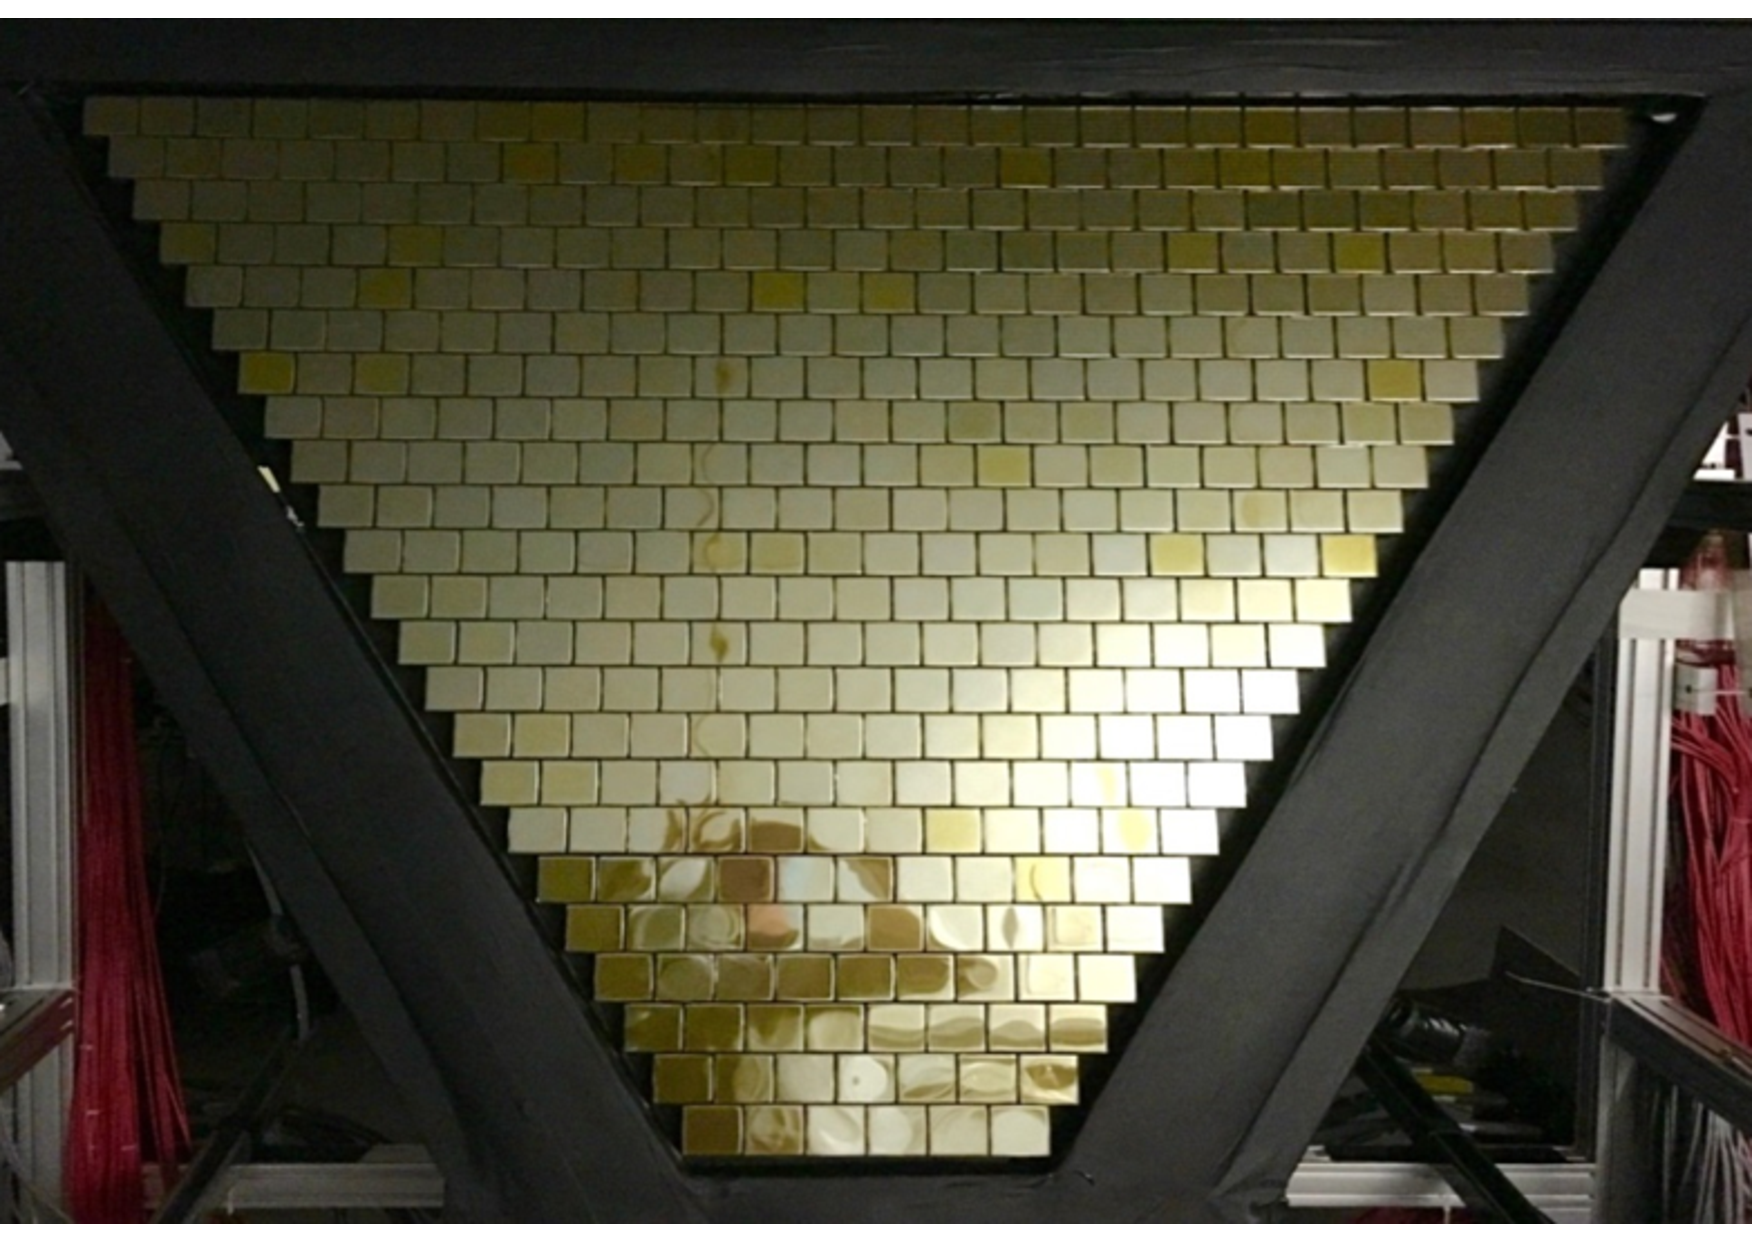
\includegraphics[width=0.4\textwidth]{EPS/mapmt.pdf}
\caption{ The plane of MAPMTs fully assembled. }
\label{fig:mapmts}
\end{center}
\end{figure}

\begin{figure}
\begin{center}
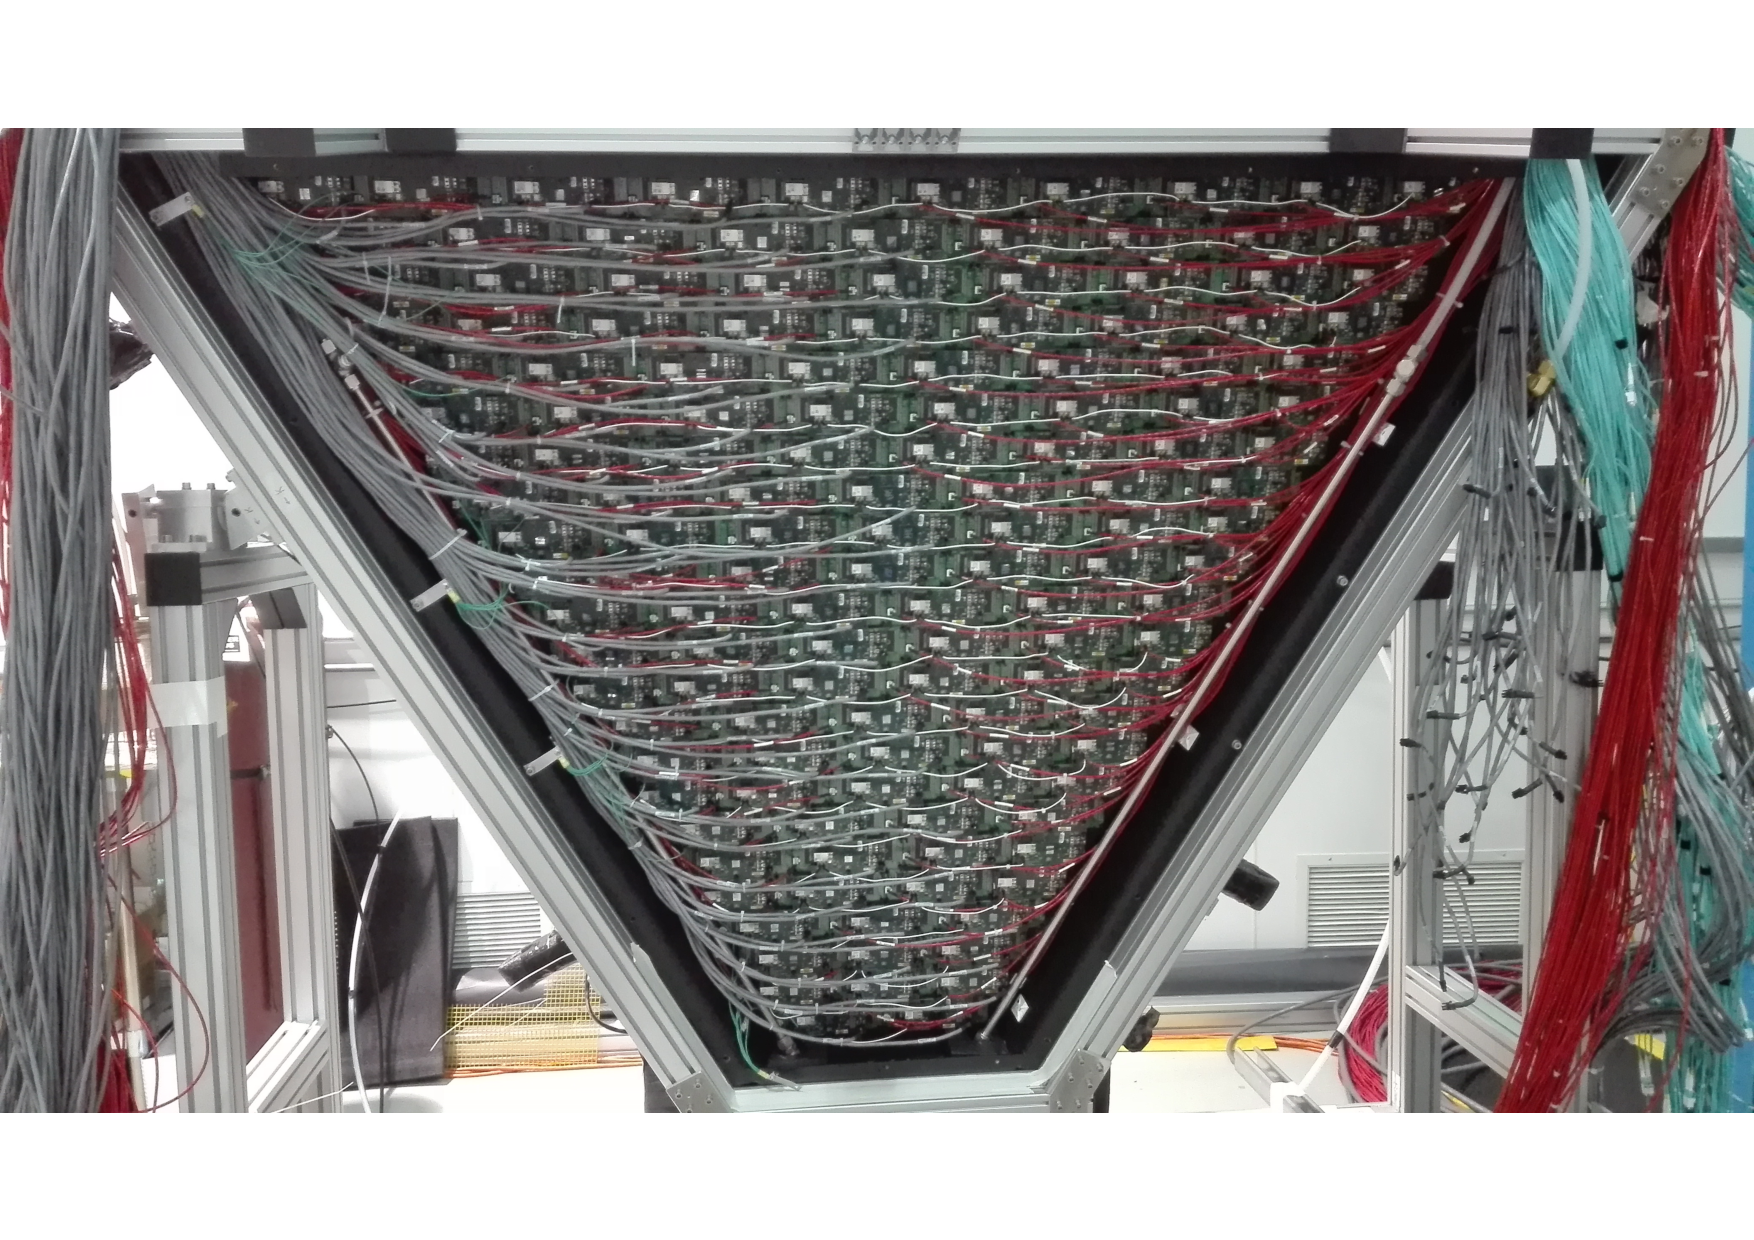
\includegraphics[width=0.45\textwidth]{EPS/electronics.pdf}
\caption{ The Front End electronics fully assembled and cabled.  }
\label{fig:electronics}
\end{center}
\end{figure}

Several tests have been performed with cosmic rays at various stages of the detector assembling. 
The photodetectors and the readout electronics were extensively tested using cosmic rays detected by a tracking system installed on
a dedicated trigger station inside a large dark box. In the absence of a precise
measure of the cosmic particle momentum it was not possible to perform a study of the Cherenkov angle resolution.
Nevertheless, cosmic runs allowed to validate the translation tables relating electronic channels with pixel positions,
develop the ring reconstruction software, verify the stability of the system, and test the performance of the services
(power supplies, cooling, readout, slow-control, interlock).

Once the detector was sealed and before the transportation to the experimental hall, its functioning parameters were tested for several
weeks in the assembly room. The tests included the two gas systems serving the RICH: the nitrogen system that must keep the internal
humidity at few percent level to preserve the optical performance of the aerogel and the air cooling system of the readout electronics.

%-----------------------------------------------
\section{Commissioning With Beam}
%-----------------------------------------------

\begin{figure}[t]
\begin{center}
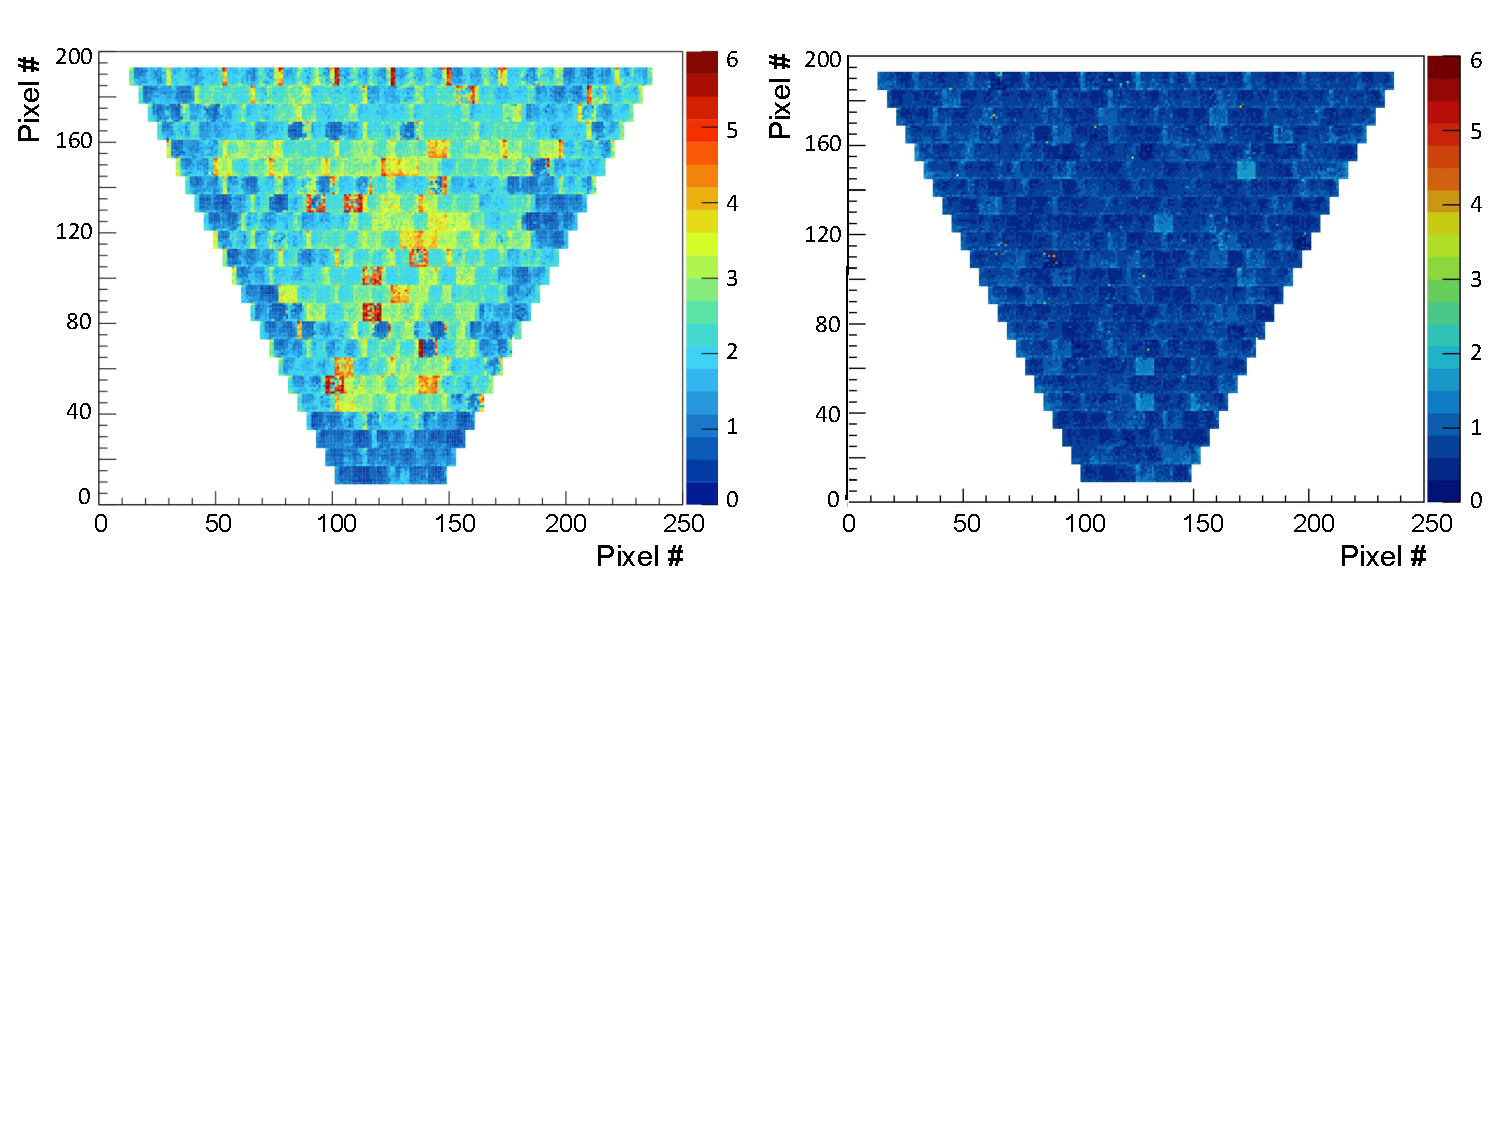
\includegraphics[width=1.0\columnwidth]{EPS/Grounding.pdf}
\end{center}
\caption{(Left) Pedestal rms values before (left) and after (right) the realization of a grounding
grid connecting all the electronic units to the RICH chassis to provide a reference for the 
floating power lines.}
\label{Fig:GroundG}
\end{figure}

\begin{figure}[t]
\begin{center}
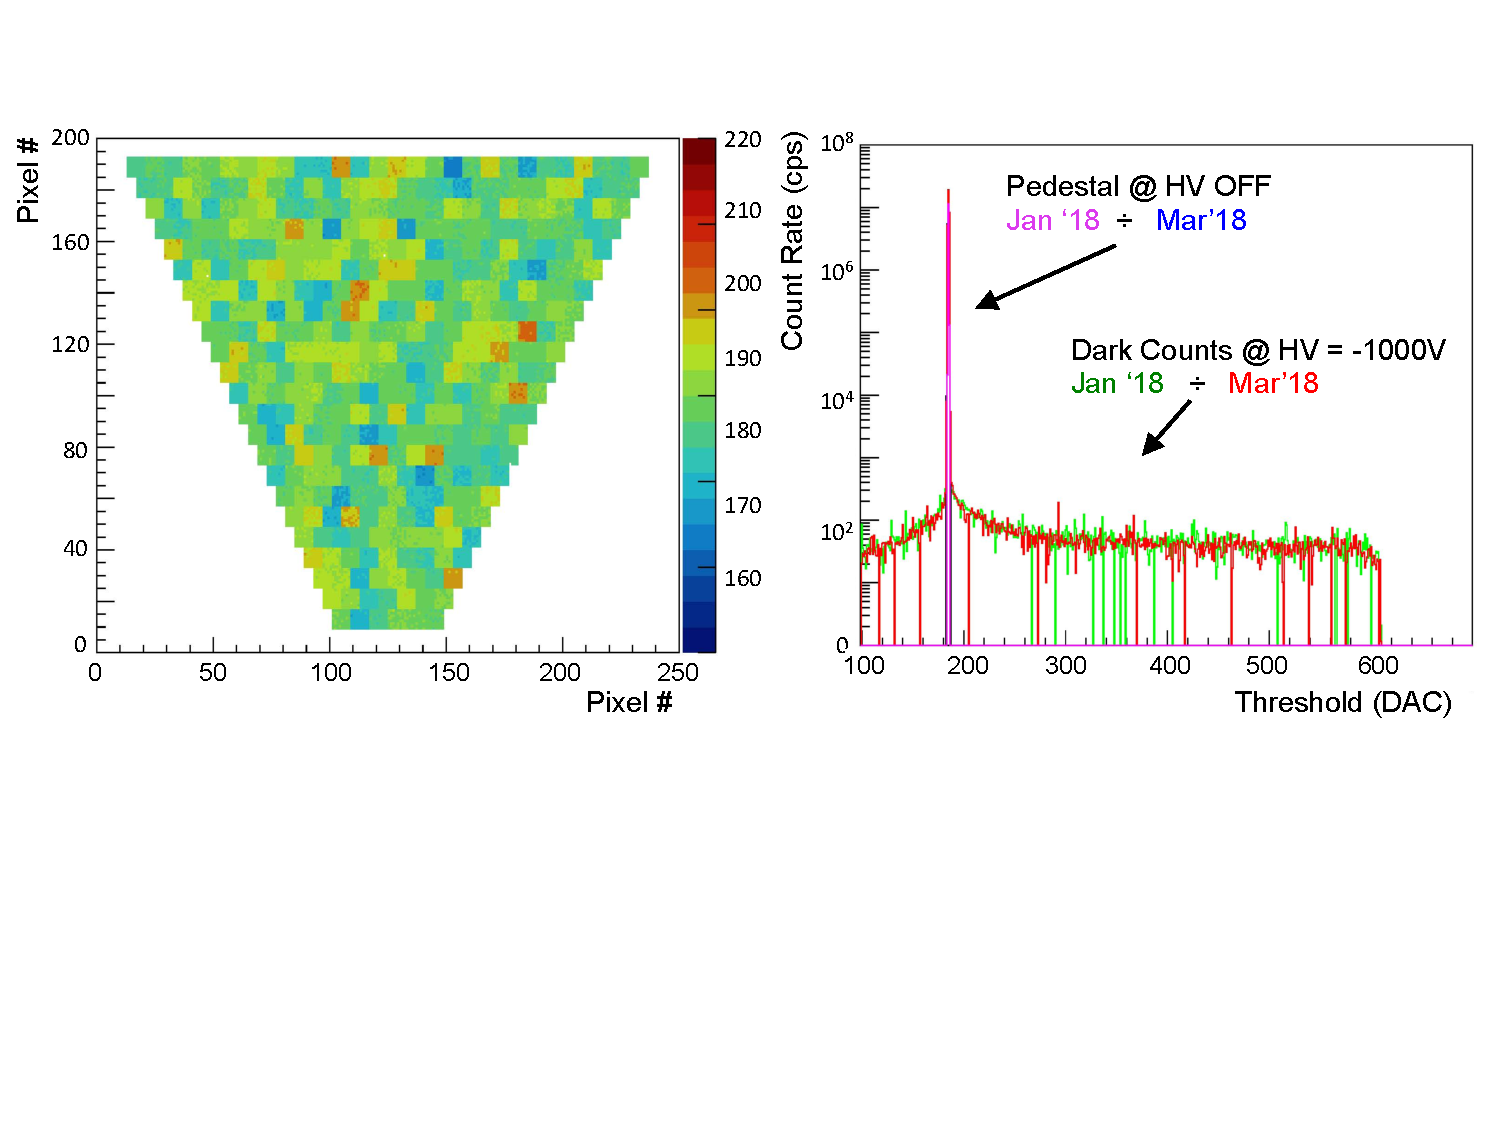
\includegraphics[width=1.0\columnwidth]{EPS/Figure5.pdf}
\end{center}
\caption{
(Left) Pedestal map of the whole MAPMT plane showing the
values within the same MAPMT are quite uniform. (Right) Count rate of one MAPMT pixel as a function of the
discrimination threshold as measured at the beginning and at the end of the first CLAS12 physics run.
A pixel with a dark count rate above the average is chosen for better visibility.
The discriminated signals have been recorded within a programmed time window at each of the thresholds selected for the scan.
The peak corresponds to the pedestal (when the threshold equals the baseline), visible also at HV OFF. The tails to the
dark count signals (bipolar after the shaping section) at HV ON. The shoulders around the pedestal are due to cross-talk
signals. The almost flat behaviour up to 600 DAC is due to the large amplification (and almost saturated
signals). The pixel behaviour is stable along the time. Color scales and threshold are in DAC units.}
\label{Fig:PedTime}
\end{figure}

The RICH detector was installed in the CLAS12 experiment at the beginning of January 2018. The electronics pedestal values 
were regularly monitored during the following engineering run and CLAS12 data-taking, as their stability is a crucial 
feature for the constant threshold readout. 

With the full detector assembled, the measured pedestal RMS was initially at the level of few DAC units.
In order to properly refer to the same ground the whole composite readout system, powered by 156 floating 5V low-voltage lines,
a grounding grid was realized connecting by a copper wire all the boards with the detector chassis. With the grid,
%to the same ground the whole composite readout system powered by a 5~V floating low-voltage,
the typical pedestal RMS was reduced to
values comparable with the ones measured in the quality assurance tests and at the limit of the readout sensitivity,
i.e. at the level of 1 DAC and thus negligible, see Fig.~\ref{Fig:GroundG}.

The pedestal level is different for each MAROC, but is relatively uniform
within one chip, a feature conforming to the common discrimination threshold, see the left plot in Fig.~\ref{Fig:PedTime}.
With HV ON, the typical measured dark count rate is around 10 Hz/pixel, in agreement with the Hamamatsu specifications.
In the right plot of Fig.~\ref{Fig:PedTime}, the measured dark rate of one pixel of a H12700 MAPMT is plotted as a function 
of the discriminating threshold with MAPMT HV OFF (0 V) and HV ON (-1000~V), at the beginning and at the end of
the first physics run. The plot shows a large region of uniform response above a very narrow pedestal (as expected from the 
laboratory characterization) that stays unchanged over time. 

A typical feature of any constant threshold readout is the time-walk, i.e. the dependence of the discrimination time 
on the signal amplitude. The time-over-threshold (ToT) derived from the recorded start and stop signal times provides a 
non-linear estimate of the charge collected at the MAPMT anode. This can be used to correct for the time-walk effect. In order to 
have an easier handling of the time-walk and ToT behavior over the ~25000 channels of the RICH detector,
an equalization of the SPE shaped pulses is desirable, in particular because the MAROC programmable threshold is 
common to all its 64 readout channels.  The RICH channel-by-channel SPE signal 
equalization was performed during the CLAS12 engineering run with real data. Data-acquisition tests were made at various 
thresholds for different MAROC gain configurations. Fig.~\ref{Fig:Equali} shows the ToT distribution for 
three typical values of the threshold: on the left for all channels without amplification (nominal MAROC gain of 1),
on the right after equalization (tuning the average MAPMT+MAROC gain to $2.7\times 10^6$ in all the channels).
After equalization, the ToT distribution of saturated SPE signals is narrower than before. With typical ToT values 
larger than 40 ns, it also is clearly separated from the cross-talk signals whose ToT values distribute around 25 ns.

\begin{figure}[t]
\begin{center}
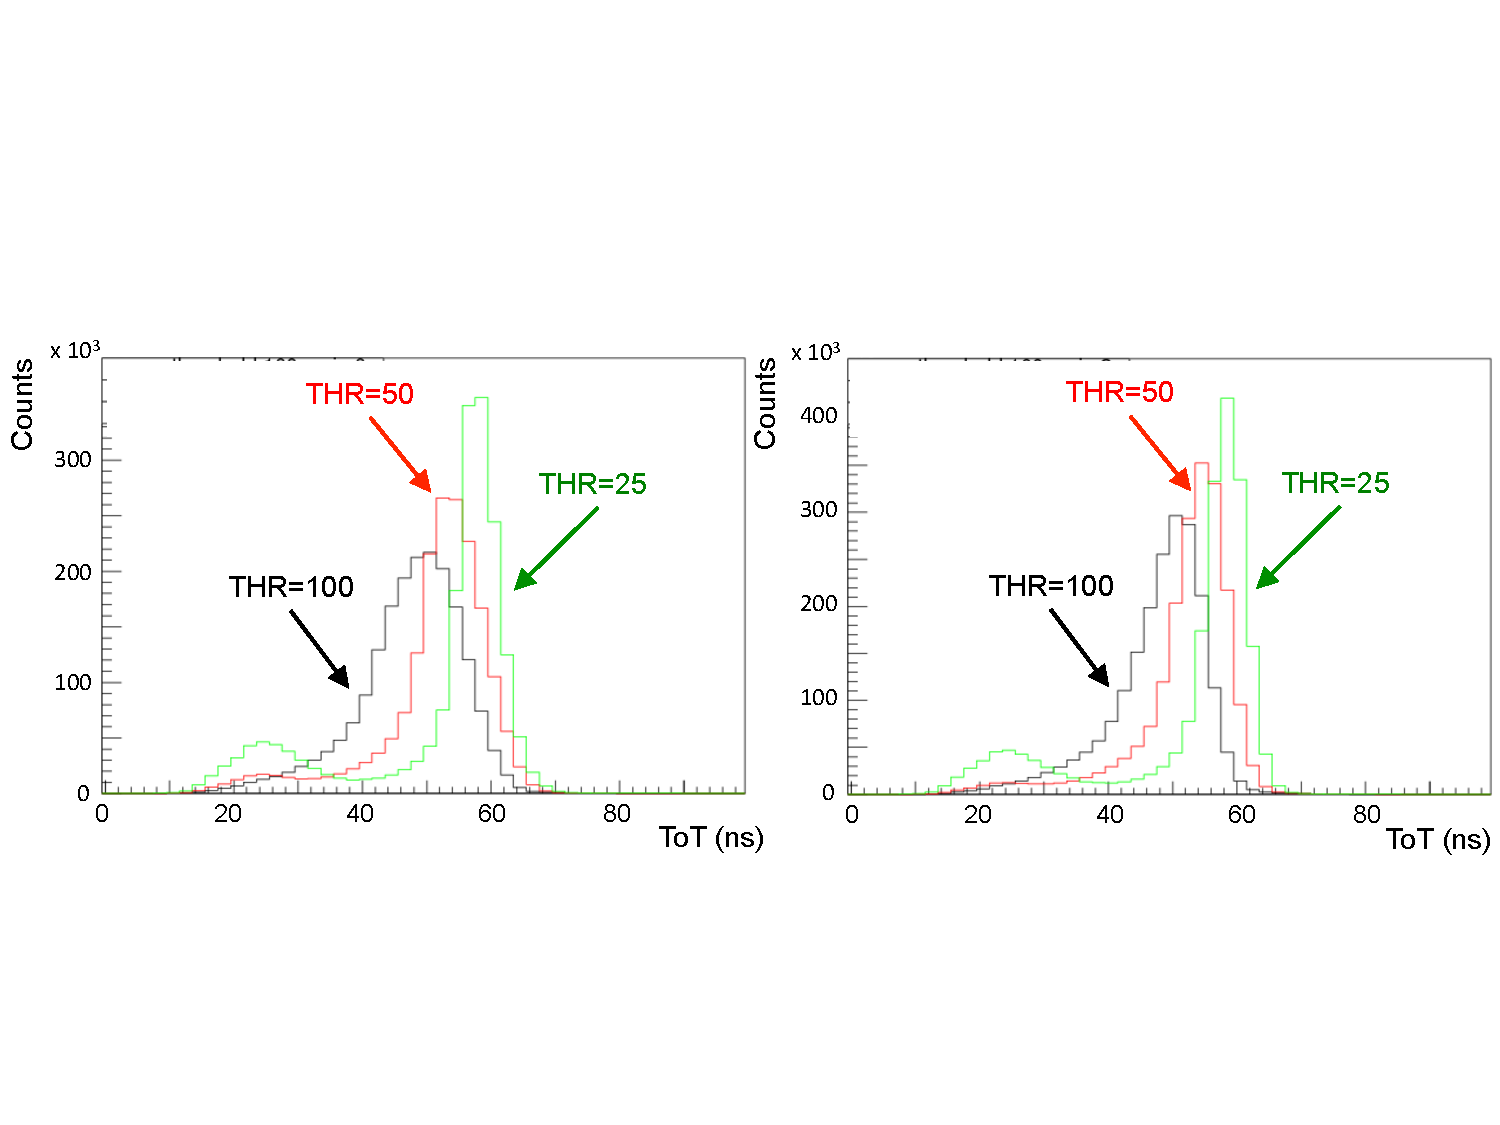
\includegraphics[width=1.0\columnwidth]{EPS/Figure6.pdf}
\end{center}
\caption{ToT distributions of the RICH channels at three typical values of 
threshold (25, 50 and 100 DAC) without (left) and with (right) gain equalization.
The saturated SPE signals generally yield ToT duration greater than 40~ns.
When lowering the threshold also weaker cross-talk signals are recorded
with ToT duration around 25~ns.}
\label{Fig:Equali}
\end{figure}

%------------------------------------------------
\section{RICH Slow Control}
%------------------------------------------------

Description and performance

\begin{figure}[t]
\begin{center}
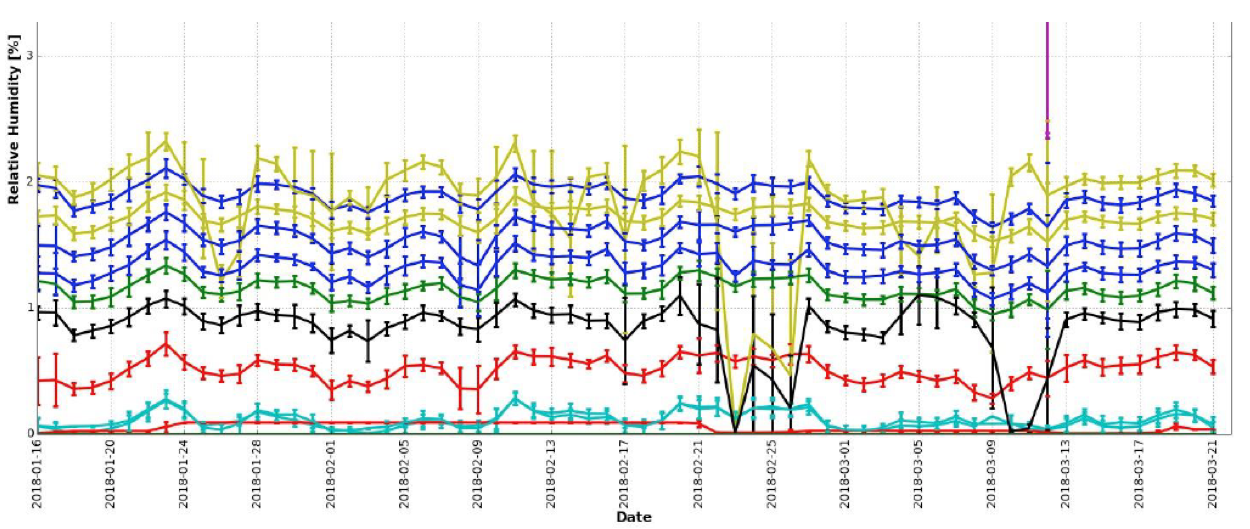
\includegraphics[width=1.0\columnwidth]{EPS/Humidity.png}
\end{center}
\caption{Monitor of the humidity level in the inner RICH volume over the three months of the first
CALS12 data-taking period. The lines (colors) correspond to different sensors positioned in 
various locations inside the RICH.}
\label{Fig:EfScan}
\end{figure}

%------------------------------------------------
\section{RICH Event Reconstruction}
%------------------------------------------------

The RICH reconstruction is organized into 4 steps. 

In the first step, the spatial and time information 
of heach hit is reconstructed taking into account possible misalignments and calibration
corrections. If more than 3 hits are found around a local maximum, they are grouped
into a RICH cluster. A cluster is tipically created by a charged particle producing
Cherenkov light into the \MAPMT window or ionization into the sensor dynode structure.
The time of the cluster is taken to be equal to the time of the local maximum, while its
spatial coordinates are calculated as a weighted average over all the hits with their 
ToT vlaue as the weight.
If a sole hit is found close to a local maximum, with an amplitude lower than 80\% of that 
maximum, the hit is flagged as possible cross-talk. The hit should be within a 3x3 \MAPMT 
pixel matrix (nonet) centered on the maximum, or on a \MAROC input adjacent to the maximum, 
to be flagged as optical or electrical cross-talk, respectively. This selection rejects about
YY\% of the cross-talks and further reduction would be only possible with a time 
versus amplitude analysis, see Fig.~\ref{Fig:Spurious}. The cross-talk selection also removes
a small 3\% fraction of true single photo-electron signals. Those correspond to SPE signals
that undergo an incomplete dynode multiplication, while being by chance close in space
to an independent standard SPE signal.
Cross-talk hits are not considered further in the RICH reconstruction.

In the second step, RICH clusters are associated to the CLAS12 tracks if a match in space
is found, i.e. the extrapolated impact point of the track into the \MAPMT plane is closer 
than 10 cm to the cluster center. Matched clusters allow a precise study of the \MAPMT
detector position and orientation relative to the CLAS12 tracking system, see Fig.~\ref{Fig:DCmatch}.

The third step is the core of the RICH reconstruction. For each hit in the MAPMT plane, an estimate of the corresponding Cherenkov 
angle is derived by ray-tracing the photon path inside the RICH volume taking into account 
possible reflections. This is done in turn for each particle traced trough the RICH,
with the photon emission point assumed to be the middle 
point of the particle path inside the aerogel radiator. 

In the forth step a particle identification algorithm is applied using an event-based likelihood
of the reconstructed Cherenkov angles.

\begin{figure}[t]
\begin{center}
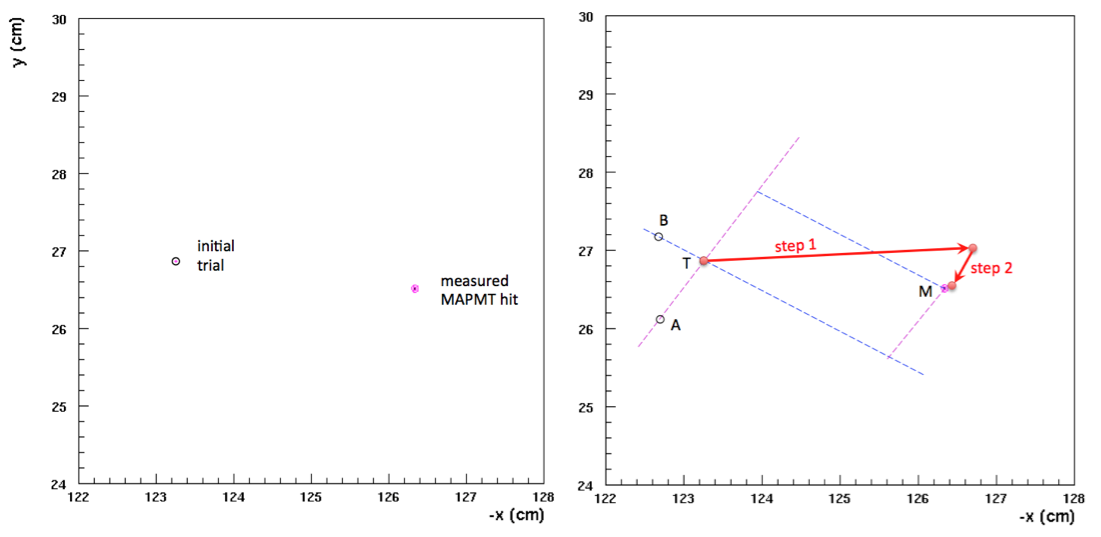
\includegraphics[width=1.0\columnwidth]{EPS/Ray-trace.png}
\end{center}
\caption{Example of the ray-tracing iterative photon path reconstruction. At each step, the
emission polar and azimuthal angles of the trial photon T are varied by the expected Cherenkov angle resolution to 
extrapolate the detection points A and B. The distance vector $\vec{TM}$ between the measured hit M and the trial T is projected
onto the displacement vectors $\vec{TA}$, corresponding to an angular shift of $\delta \theta$, to estimate the scale factor 
$f$ of the wanted angular step $\Delta \theta = f \delta \theta$ with $f=(\vec{TM}\cdot \vec {TA}) / |\vec{TA}|^2$. The
same is done for the azimuthal angle $\phi$.} 
\label{Fig:RayAlgo}
\end{figure}

The photon path inside the RICH is reconstructed in two complementary ways. The first is an analytic formula that takes into account
the refraction at the aerogel face and is only valid for directly detected photons. It provides an 
exact solution that derives the correct aerogel refractive index in conjunction with the reconstructed
Cherenkov angle. The second is a ray tracing algorithm that takes into account also the mirror reflections.
The relevant RICH components (aerogel, mirrors, \MAPMT plane) are converted into ray-tracing planes or 
spheres where the phtoon undergoes refraction, reflection or detection. 

Each ray-tracing element can be independently aligned. The alignment procedure uses as benchmark the 
Cherenkov signal generated by particles identified as electrons by CLAS12 subdetectors other than RICH. 
For these particles, the expected Cherenkov angle is given by the known particle momentum and mass. The 
position and orientation of the \MAPMT plane is defined by minimizing the average matching distance of the
RICH clusters from the extrapolated DC tracks. Each other RICH ray-tracing element can be aligned with respect to the 
\MAPMT plane by selecting the sub-sample of photons passing through that component. The alignment is made by minimizing 
the average distance between the ray-traced detection point (rdp) and the corresponding measured \MAPMT hit over the 
selected sub-sample of photons.

\begin{figure}[t]
\begin{center}
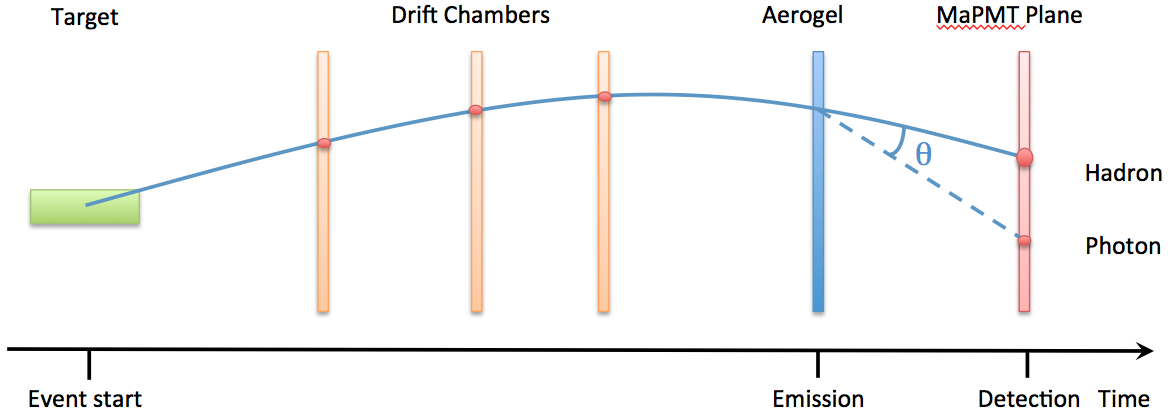
\includegraphics[width=1.0\columnwidth]{EPS/Tracking_time.png}
\end{center}
\caption{The photon detection time as mesured by the RICH can be compared to the more precise time extrapolated
by the CLAS12 spectrometer. The latter is defined as the event start time plus the fligh-times of the hadron 
from the interaction point to the radiator center, and of the ray-traced photon within the RICH volume. Any systematic
difference emerging as the average over several events provides a mean of calibration for the RICH time. After calibration,
a time coincidence within the event can be used to validate the single photon reconstructed path and emission point.}
\label{Fig:Traced_Time}
\end{figure}

For each hadron track, the ray-tracing algorithm progresses as described in the following. A limited ensamble of 
hypothetical photons (about 50) is traced assuming an initial particle hypothesis (electron for a particle identified 
as electron in CLAS12, pion otherwise). These photons, called trials, are assumed to originate at the
emission point at a Cherenlov angle $\theta_0$, corresponding to the given particle hypothesis, and at an azimuthal angle
$\phi_0$, uniformily distributed around the charged particle trajectory.
Their ray-traced detection points provide a reference path for the reconstruction. 
For each \MAPMT measured hit, the closest rdp at a distance smaller than 10 cm is taken to be the starting point of the ray-tracing procedure for that hit.
An estimate of the angular distance between the trial and measured photon $\Delta \theta = f \delta \theta$ is
estimated by ray-tracing a test photon with the angle $\theta=\theta_0 + \delta \theta$ varied 
by the SPE angular resolution $\delta \theta$. On the \MAPMT plane, an estimate of the factor $f$ can be obtained
as the scalar product of the vector connecting the trial to the measured hit with the 
vector connecting the trial to the test rdp, see Fig.~\ref{Fig:RayAlgo}. A negative $f$ signals a wrong choice of the test direction. 
The same is done for the azimuthal $\phi$ angle. 
A new trial photon is traced with the angles changed by such calculated angular shifts 
($\theta_0 + \Delta \theta$, $\phi_0 + \Delta \phi$) and the procedure
repeated. At each step the trial rdp gets closer to the measured hit, but an exact solution can 
not be found as the procedure uses a linear approximation relating the distances in the \MAPMT plane with 
the angular shifts in the 3D space. The iterative procedure stops when 
the distance of the trial rdp to the measured hit is smaller than half of the \MAPMT pixel size (RICH detector spatial resolution).
The converge is fast, typically within 3 steps.

\section{RICH Time Calibration}

The reconstructed photon path and angle are validated by a $\pm 3\sigma$ ns time coincidence between the RICH 
recorded time and the CLAS12 expected time, where $\sigma$ is the estimated single photon-electron time resolution, 
see Fig.~\ref{Fig:Traced_Time}. The expected time is defined as the event start time of the 
beam particle primary interaction with the target plus the flight time of the produced hadron to the aerogel 
radiator and of the ray-traced photon to the sensor.
The CLAS12 expected time much smaller time uncertainty than RICH, 
being defined by a precise time-of-flight system with better than 0.1 ns time precision corrected
with the beam radio-frequency clock~\cite{Ref:CLASTOF}. The hadron tracjectory is calculated taking into account the magnetic field 
inhomogeneities and fringes~\cite{Ref:CLASDC}.

The difference \dT of the RICH measured time from the more precise CLAS12 extrapolated time provides a practical way to 
calibrate the RICH time, estimate the RICH time resolution and identify spurious signals, see Fig.~\ref{Fig:Spurious}. 

\begin{figure}[t]
\begin{center}
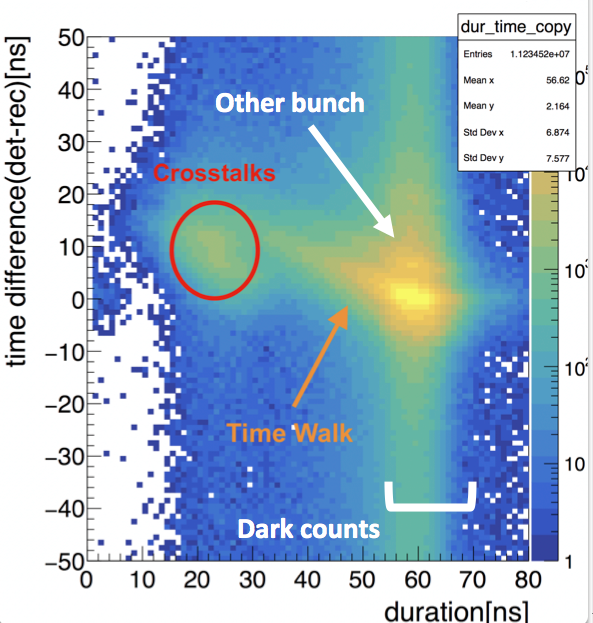
\includegraphics[width=0.6\columnwidth]{EPS/Spurious_Components.png}
\end{center}
\caption{Typical online plots showing the cumulative distribution of the difference \dT between RICH measured 
and CLAS12 extrapolated times as a function of the hit duration. Several features are highlighted. 
Single photo-electron \MAPMT discharges concentrate at 60 ns duration. The single channel time-offsets result in 
a broad peak of Chrenkov signals around \dT equal zero, whereas the off-time band corresponds to random dark counts
or wrong beam bunches. The time-walk of small SPE signals, generated by the constant threshold readout, is visible 
as a drifting tail at smaller duration times. An independent excess around 20 ns duration times signals a residual 
contamination of cross-talk signals.}
\label{Fig:Spurious}
\end{figure}

The cumulative \dT distribution over several events is used to measure and monitor the time-offset of each of the 25 thousands
RICH readout channels, see Fig.~\ref{Fig:TimeOff}. Individual time-offsets are due to the specific front-end chip performance, readout 
circuit routing and data-acquisition fiber-optic length, in conjunction with the configuration details of the CLAS12 trigger 
distribution system which may vary during the data-taking.

\begin{figure}[t]
\begin{center}
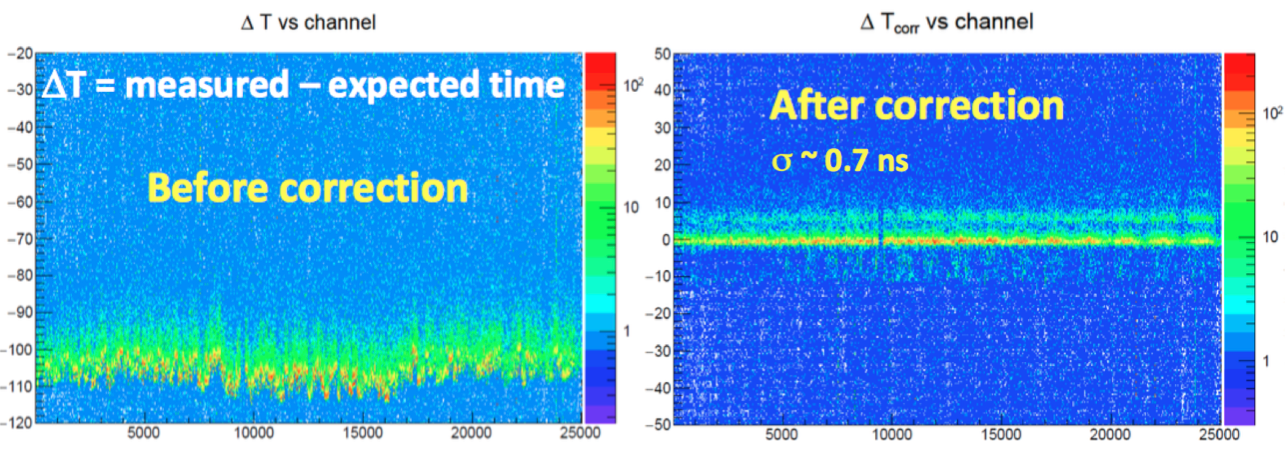
\includegraphics[width=1.0\columnwidth]{EPS/Time_correction.png}
\end{center}
\caption{Distribution of the time difference \dT between measured RICH and extrapolated CLAS12 times as a function 
of the RICH readout channel. On the left before and on the right after the RICH time-offset calibration.}
\label{Fig:TimeOff}
\end{figure}

The dependence of \dT over the signal duration time is fitted to extract the time-walk dependence. The fit
assumes two linear dependences with different slopes, one in the saturated region around 60 ns duration times, 
one for unsaturated signals at smaller duration times. The exact point separating the two regimes is also
defined by the fit. The time-walk is a feature of the constant threshold readout and ultimately depends
on the intrinsic MAROC3 shaping signal configuration. As a consequence, it is not expected to vary over the 
\MAPMT channels readout by the same chip, and to not depend on the data-acquisition and trigger 
distribution configuration details. This features has been validated by data. Despite the time-offsets change with
the run conditions, the time-walk appear to be relatively stable during the data-taking. Being almonst independent
by the single channel behaviour, the time-walk fit is done at \MAPMT level, integrating the signals of all
the pixels.

\begin{figure}[t]
\begin{center}
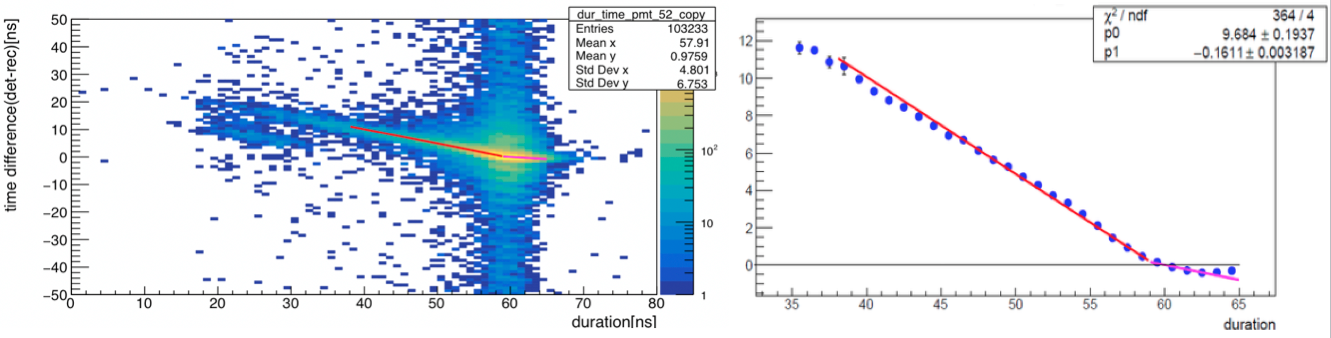
\includegraphics[width=1.0\columnwidth]{EPS/Time_walk_corr.png}
\end{center}
\caption{Example of time-walk correction. On the left the distribution of photon signals after the time-offset
calibration. The fit function is highlighted in red. On the right the detail of the fit, performed over the
average time values calculated in bins of time duration.}
\label{Fig:TimeOff}
\end{figure}


\section{Performance During the Physics Run}

After calibration, the typical time resolution is of the order of 0.7 ns and well within the RICH specification 
to be less than 1 ns, see Fig.~\ref{Fig:Resos}. Such a time resolution is instrumental to suppress the spurious signals highlighted in 
Fig.~\ref{Fig:Spurious}, and to identify direct and reflected photon paths. A photon that is reflected back by 
the spherical mirror, and undergoes a second reflection towards the photon detector, travel a distance almost
three times longer than a direct photon, resulting in a time difference of the order of 6 ns. 

\begin{figure}[t]
\begin{center}
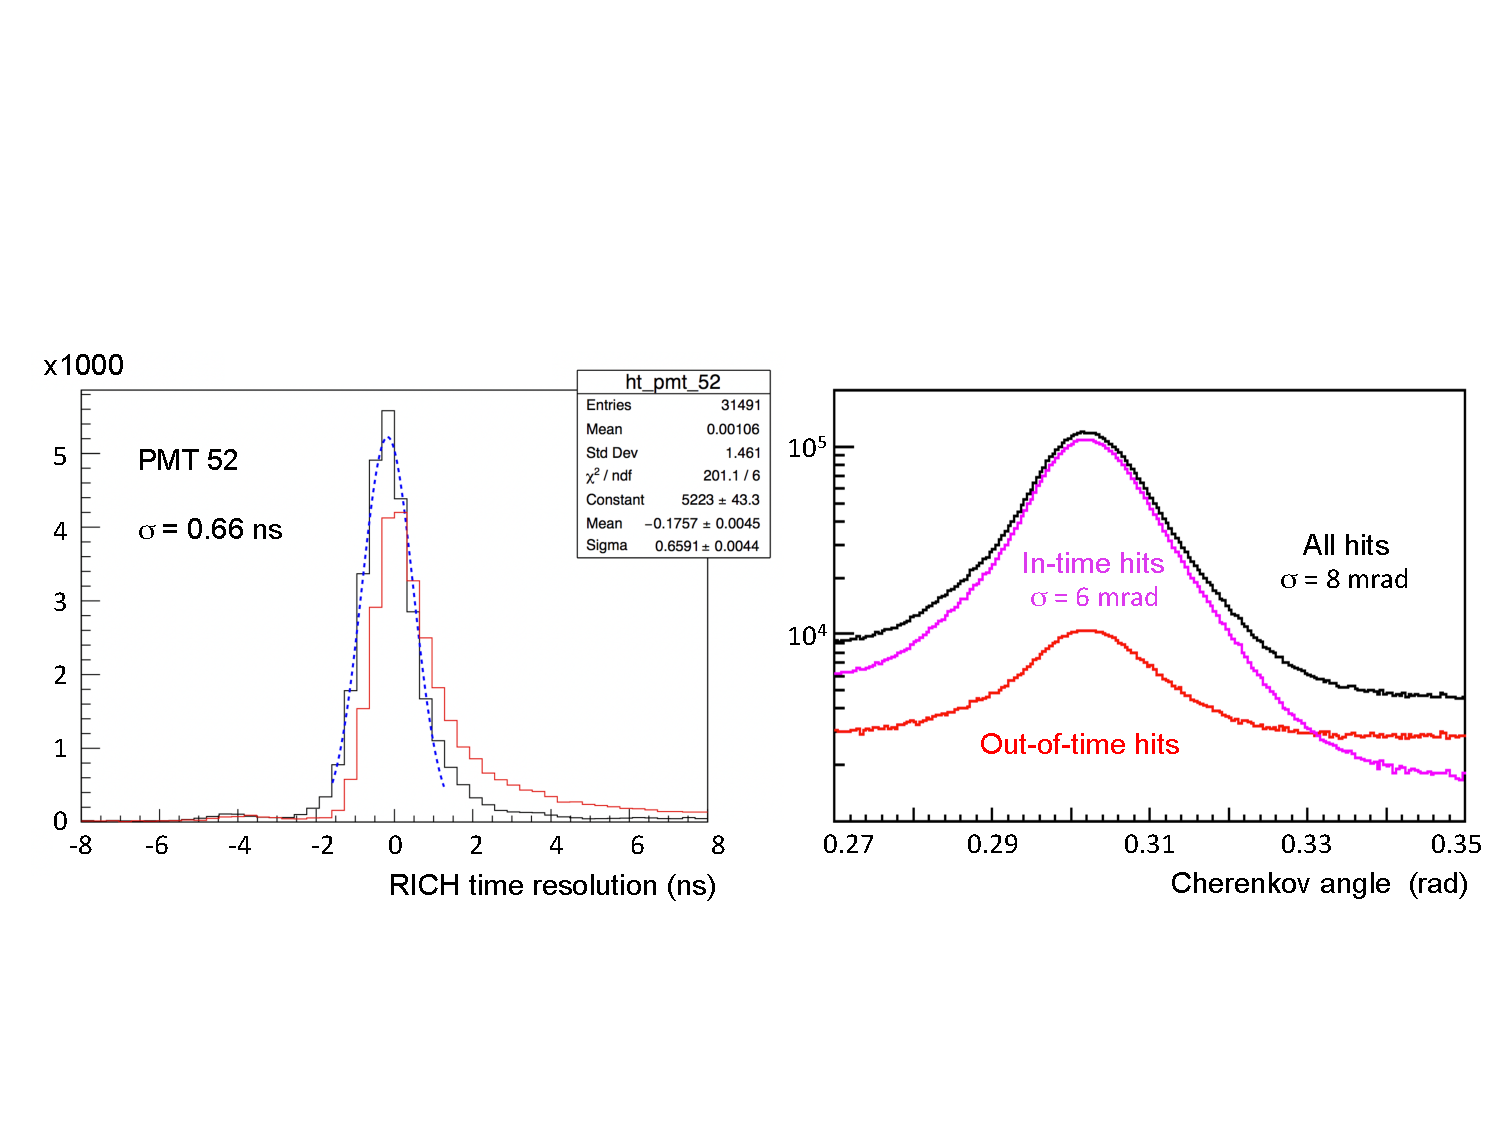
\includegraphics[width=1.0\columnwidth]{EPS/Figure8.pdf}
\end{center}
\caption{(Left) Typical time resolution before (red) and after (blue) time-walk correction for all the pixels in 
MAPMT 52. (Right) Cherenkov angle reconstruction without (black) and with (magenta) a time coincidence request 
between RICH detected and CLAS tracking times (the difference is in red).}
\label{Fig:Resos}
\end{figure}

Examples of reconstructed RICH events are shown in Fig.~\ref{Fig:Events}. A remarkable feature is the low level
of spurious hits from accidentals, in-time background (i.e. Rayleigh scattering) and dark counts. This feature
is crucial for the most challenging cases: particles with high momenta close to the 8 GeV limit that require
the best resolution in Cherenkov angle, and particles pointing towards the spherical mirror whose number of
detected photons is limited by the double reflection and a second passage through the radiator. 

\begin{figure}[t]
\begin{center}
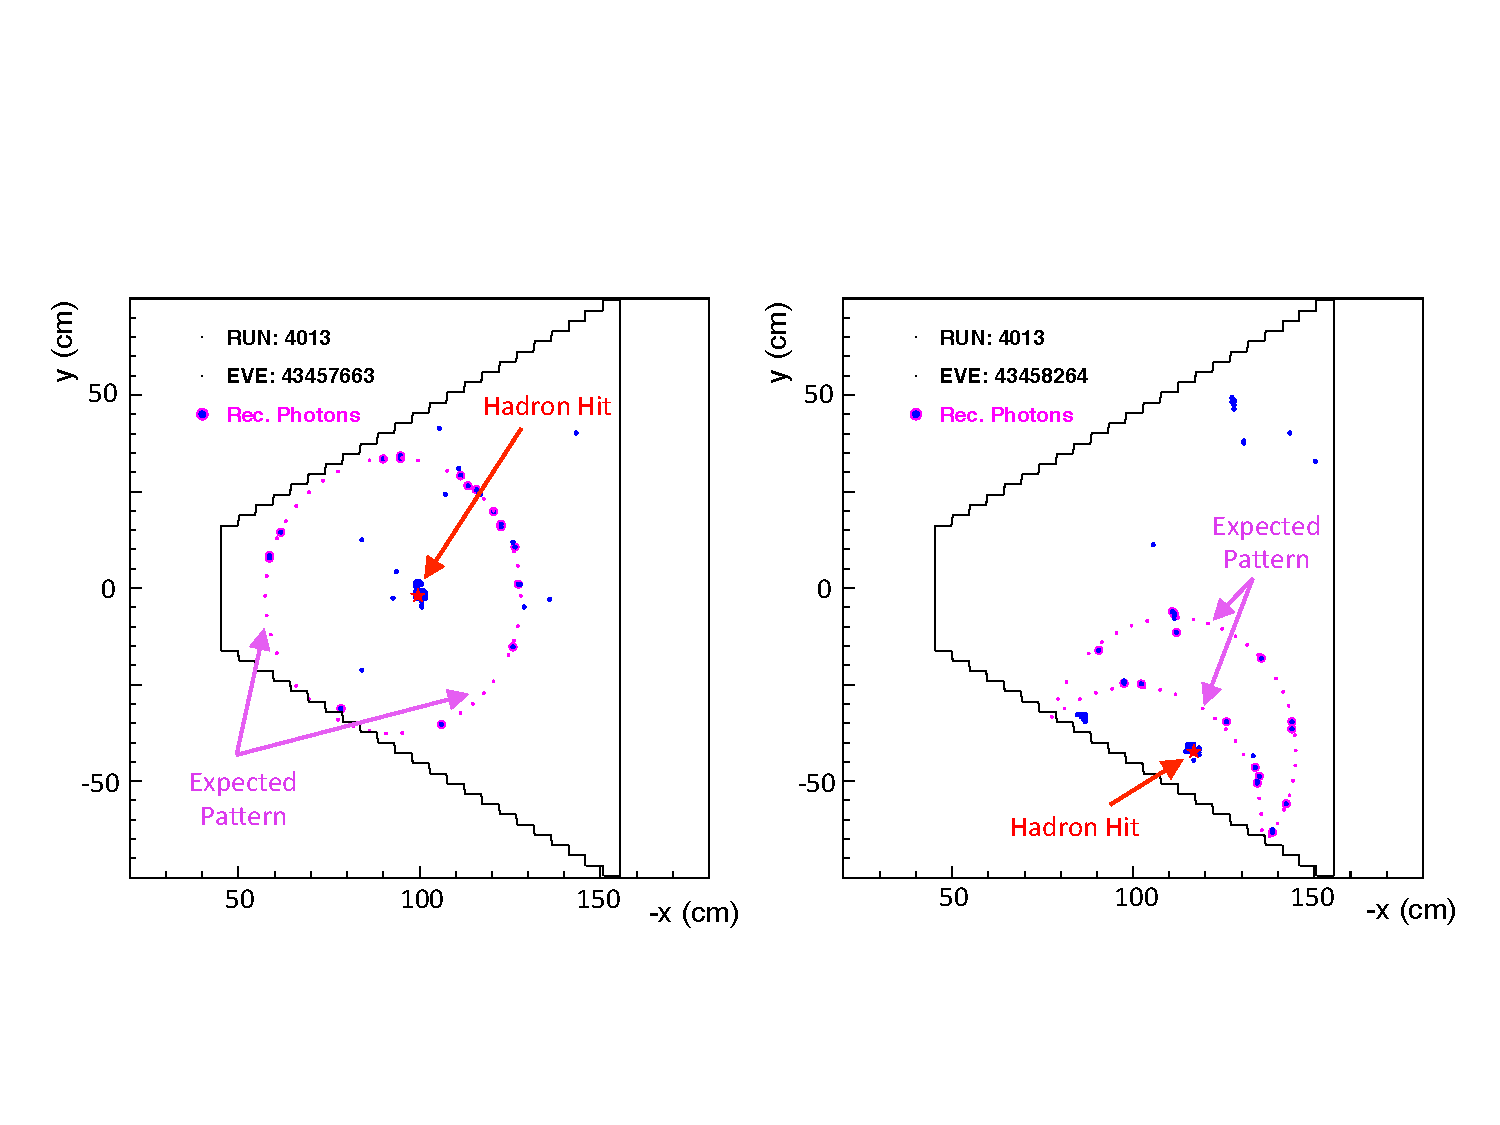
\includegraphics[width=1.0\columnwidth]{EPS/Figure7.pdf}
\end{center}
\caption{Examples of RICH reconstructed events: direct (left) and partially reflected (right). Big dots indicate
the reconstructed photon hits. The arrows indicate
the hadron impact point (red star) and the expected photon pattern (small magenta points).}
\label{Fig:Events}
\end{figure}

Each aerogel tile presents specific features because the challenging production process, tuned to achieve
the highest transparency over a large volume, is not fully industrialized. The most important quality 
parameters are the density, related to the average refractive index, homogeneity, related to the 
refractive index variations within the volume, and tile bending, originated by the inner material tension 
and related to the surface planarity. The effect of these features to the RICH reconstruction can 
be studied in details using the control sample of electrons identified by CLAS12. In the 2 to 8 GeV/c 
momentum range relevant for RICH, the Cherenkov cone generated by an electron is saturated to the maximum 
aperture angle corresponding to the low mass of the particle. Given the large number of tiles and the
broad range of particle directions after the CLAS12 bending magnets, such a study requires a large
statistics and is still ongoing. A similar approach is used for the alignment study. Also in this case,
a large statistics is needed due to the numerous involved components (aerogel layers, mirrors and \MAPMT
plane) and photon path configurations. Despite the above studies have not been finalized yet, and
only partial corrections have been implemented so far, the
preliminary SPE Cherenkov angle resolution yields about 6 mrad, see Fig.~\ref{Fig:Resos}. It is expected 
to improve towards the goal value of 4.5 mrad once the corrections for the detector misalignment will
be implemented and the realistic optical parameters of each aerogel tile will be accounted for. 
As an example, the effect of a preliminary alignment of the whole RICH detector (not taking into 
account possible single component misalignments) is shown in Fig.~\ref{Fig:Align}.

\begin{figure}[t]
\begin{center}
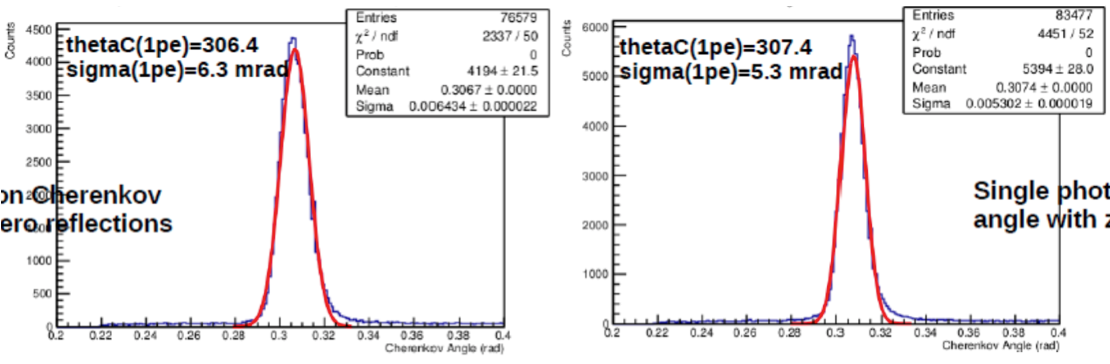
\includegraphics[width=1.0\columnwidth]{EPS/Reso_align.png}
\end{center}
\caption{RICH Cherenkov resolution before (left) and after (right) a preliminary RICH alignment.
The whole RICH detector is aligned minimizing the matching distance between RICH clusters 
and extrapolated DC tracks. No possible misalignment of the single RICH component is accounted for.
The distribution is for particles passing through one aerogel tile of 2 cm thickness (tile 12
in layer 1) and for direct photons.}
\label{Fig:Align}
\end{figure}

As a general approach, the RICH performance is studied separately for each aerogel tile, see Fig.~\ref{Fig:Tile}.
The RICH global performance estimators are then defined by averaging the results over
all the radiator tiles. The preliminary Cherenkov angle resolution resolution is already sufficient
for a effective hadron separation in the goal range of momenta, from 3 to 8 GeV/c, as shown 
by Fig.~\ref{Fig:CHele} and Fig.~\ref{Fig:CHhad}. 

\begin{figure}[t]
\begin{center}
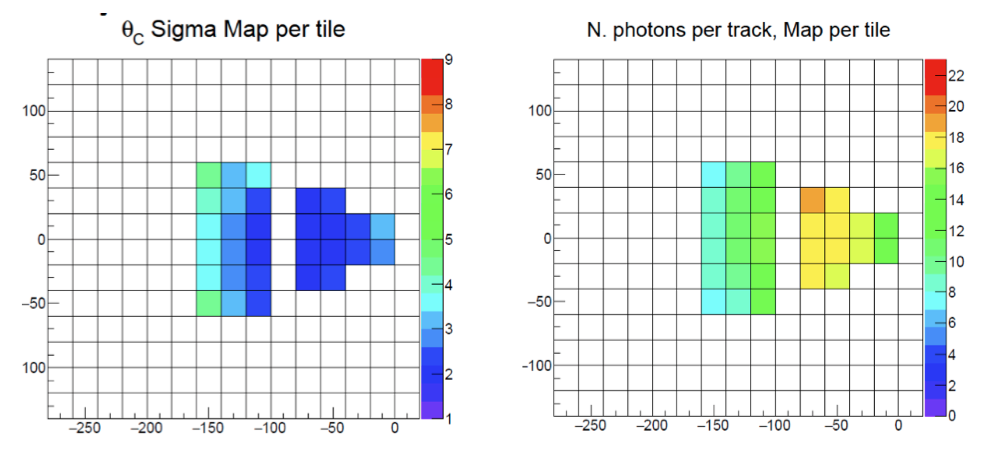
\includegraphics[width=1.0\columnwidth]{EPS/Tile_analysis.png}
\end{center}
\caption{Example of a tile dependent analysis for the aerogel of 2 cm thickness. Average number 
of reconstructed photons (left). Average Cherenkov angle resolution (right).}
\label{Fig:Tile}
\end{figure}




\begin{figure}[t]
\begin{center}
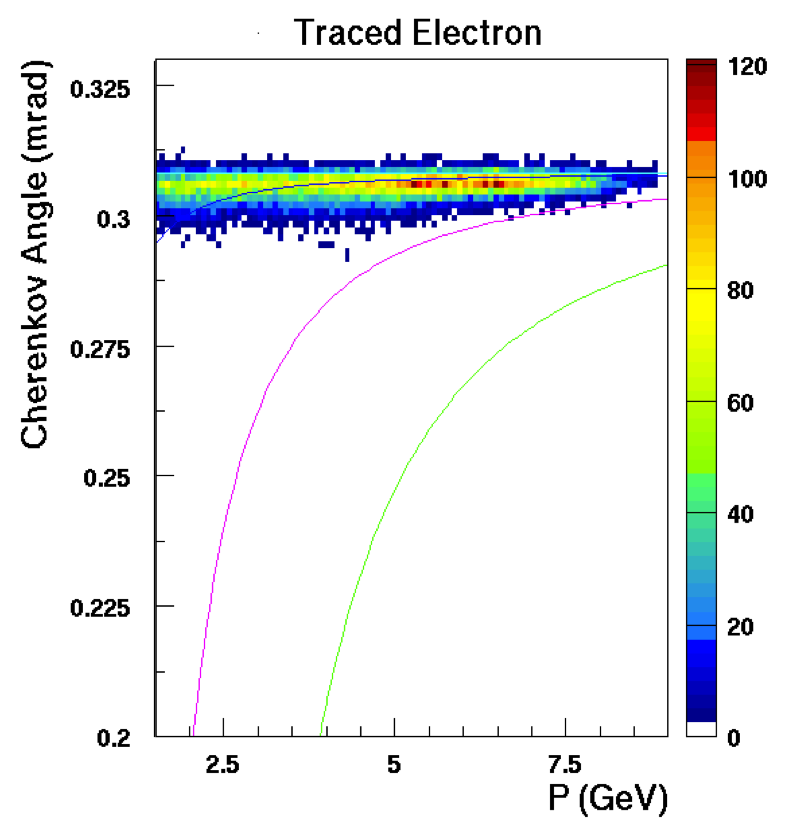
\includegraphics[width=0.55\columnwidth]{EPS/Electron_PID.png}
\end{center}
\caption{RICH response for electron particles as identified by CLAS12. As expected, the measured Cherenkov angle
is saturated over the whole momentum range, from 3 GeV/c up to 8 GeV/c. The distribution is for particles
passing through one aerogel tile of 2 cm thickness (tile 12 in layer 1) and direct photons.}
\label{Fig:CHele}
\end{figure}

\begin{figure}[t]
\begin{center}
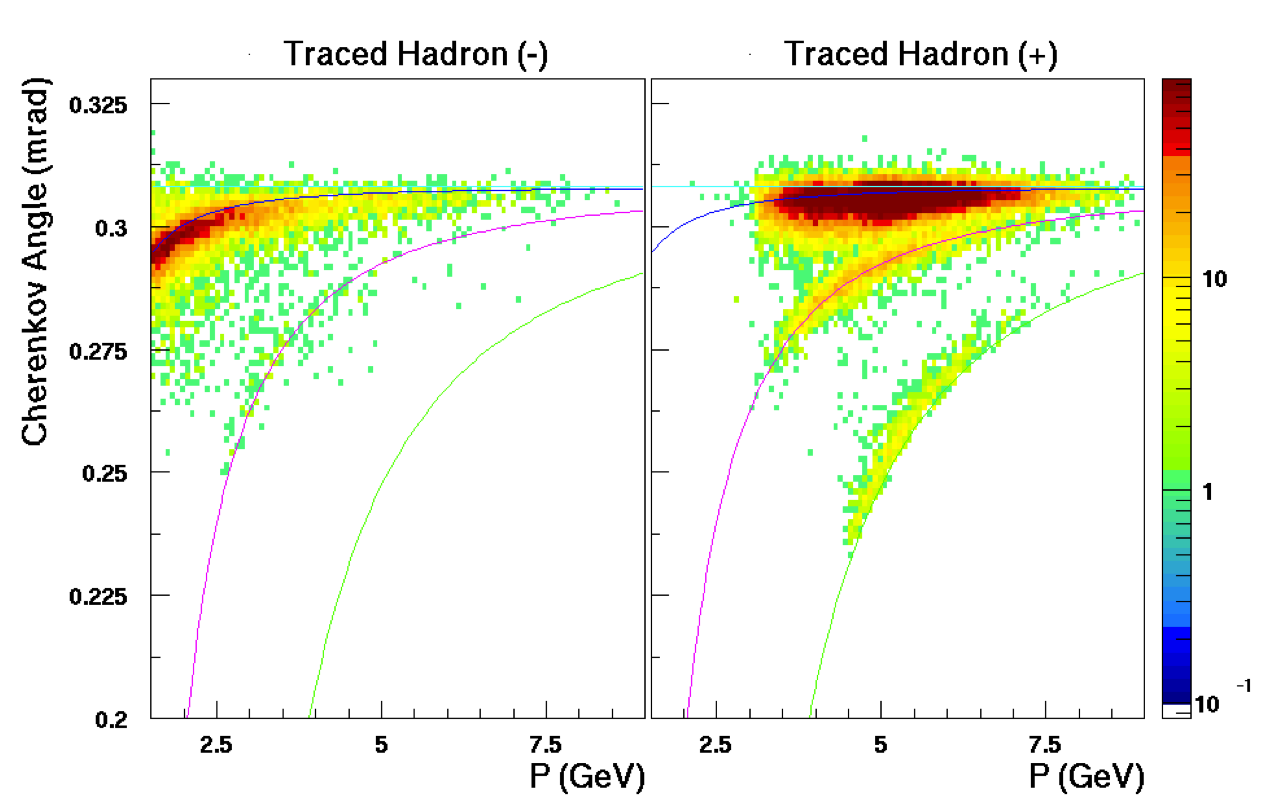
\includegraphics[width=1.0\columnwidth]{EPS/Hadrons_PID.png}
\end{center}
\caption{RICH response for non-electron particles as defined by CLAS12. The measured Cherenkov angles
distribute around the expected pion, kaon and proton values depending on the momentum. The three 
hadron population are separated over the whole momentum range, from 3 GeV/c up 
to 8 GeV/c. The distribution is for particles passing through one aerogel tile of 2 cm thickness (tile 12 
in layer 1) and direct photons resulting in a peculiar momentum distribution.}
\label{Fig:CHhad}
\end{figure}




\section{Conclusions}

Preliminary data analysis shows that the CLAS12 RICH,
for the first time equipped with H8500 and H12700 MAPMTs, is able to match the required time and Cherenkov angle resolution.
A compact and scalable readout electronics system has been realized for the detector, able to work in 
the single-photon regime with high efficiency and stability. 
%Preliminary RICH data analysis shows that, in 
%conjunction with Hamamatsu H8500 and H12700 MAPMTs, is able to match the required time and Cherenkov angle resolution.
It provides a reliable readout system for a variety of cutting-edge sensors, from densely packed H13700 MAPMTs
to novel SiPM matrices. 

\section{Acknowledgments}

%\vspace{0.2cm}
This material is based upon work supported by INFN, Italy and by the U.S. Department of Energy, Office of Science, Office
of Nuclear Physics under contract DE-AC05-06OR23177 and the National Science Foundation, Award \#1615067. We thanks the JLab Detector Support
Group and Fast Electronic Group, the Hall-B technical and management staff and the INFN technical and administrative
service.


\begin{thebibliography}{00}

\bibitem{CLAS12:tdr} CLAS12 Technical Design Report, version 5.1 208 (2008).
\bibitem{CLAS12:physics} J. Dudek {\it et al.}, Eur.Phys.J. {\bf A48} (2012) 187.
\bibitem{PSHP10} H.~Avakian \etal, {\em arXiv:1202.1910v2} {\bf [hep-ex]} (2012).
\bibitem{RICH:first} M.~Contalbrigo \etal, {\em Nucl. Instrum. Meth.} {\bf A 639} (2011) 302.
\bibitem{RICH:ElAlaoui} A.~El~Alaoui \etal, {\em Physics Procedia} {\bf 37} (2012) 773.
\bibitem{RICH:CERN} S.~Anefalos~Pereira \etal, {\em Eur. Phys. J. A} {\bf 52} (2016) 23.
\bibitem{REF:Tecnavan} http://www.tecnavan.it/en/
\bibitem{REF:Aerogel} R. De Leo {\it et al.}, Nucl. Instrum.Meth. {\bf A 595} (2008) 19; A. Yu. Barnyakov {\it et al.}, Nucl. Instrum. Meth. {\bf A 453} (200
0) 326; R. Pereira {\it et al.}, Nucl. Instrum. Meth. {\bf A 639} (2011) 37; R. Forty {\it et al.}, Nucl. Instrum. Meth. {\bf A 623} (2010) 294.
\bibitem{REF:Belle} T. Iijima {\it et al.}, Nucl. Instrum. Meth. {\bf A 598} (2009) 138.
\bibitem{RICH:RICH2016mc} M. Contalbrigo {\it et al.}, Nucl. Instrum. Meth. {\bf A876} (2017) 168.
\bibitem{Hunt} E.~Aschenauer  {\it et al.}, Nucl. Instrum. Meth. {\bf A 440} (2000) 338.
\bibitem{REF:CMA} http://www.compositemirrors.com/
\bibitem{REF:ECI} https://www.evaporatedcoatings.com/
\bibitem{REF:MediaLario} http://www.media-lario.com/

\bibitem{Ref:H8500} https://www.hamamatsu.com/resources/pdf/etd/H8500\_H10966\_TPMH1327E.pdf.
\bibitem{MAPMT:test} R.~A. Montgomery \etal, {\em Nucl. Instrum. Meth.} {\bf A 695} (2012) 326.
\bibitem{Ref:H12700} https://www.hamamatsu.com/resources/pdf/etd/H12700\_TPMH1348E.pdf.
\bibitem{MAROC3:chip} S. Blin \etal, {\em IEEE Nucl. Sci. Symp. Conf. Rec. 2010} (2010) 1690.
\bibitem{MAPMT:laser} M.~Contalbrigo \etal, {\em Nucl. Instrum. Meth.} {\bf A 787} (2015) 224.
\bibitem{MAPMT:model} P.~Degtiarenko, arXiv:1608.07525.
\bibitem{Ref:GlueX} F.~Barbosa \etal, {\em Nucl. Instrum. Meth.} {\bf A 876} (2017) 69. 
\bibitem{Ref:mRICH1} C.P.~Wong \etal, {\em Nucl. Instrum. Meth.} {\bf A 871} (2017) 13. 
\bibitem{Ref:eRD14} A.~Del~Dotto \etal, {\em Nucl. Instrum. Meth.} {\bf A 876} (2017) 237.
\bibitem{Ref:H13700} https://www.hamamatsu.com/resources/pdf/etd/H13700\_TPMH1370E.pdf.
\bibitem{Ref:MPPC} https://www.hamamatsu.com/resources/pdf/ssd/s13361-3050\_series\_kapd1054e.pdf.

\bibitem{Ref:CLASTOF} D. Carman \etal, {\em This volume}
\bibitem{Ref:CLASDC} M. Mayster \etal, {\em This volume}

%\bibitem{Past:rich} R. De Leo \etal, {\em Nucl. Instrum. Meth.} {\bf A 595} (2008) 19;
%A.~Yu. Barnyakov \etal, {\em Nucl. Instrum. Meth.} {\bf A 453} (2000) 326;
%R. Pereira \etal, {\em Nucl. Instrum. Meth.} {\bf A 639} (2011) 37;
%R. Forty \etal, {\em Nucl. Instrum. Meth.} {\bf A 623} (2010) 294.
%\bibitem{Belle:rich} T. Iijima \etal, {\em Nucl. Instrum. Meth.} {\bf A 598} (2009) 138.
%\bibitem{budker:aerogel} A.~Yu. Barnyakov \etal, {\em Nucl. Instrum. Meth.} {\bf A 639} (2011) 225.
%\bibitem{aerogel:clarity} T. Bellunato \etal, {\em  Nucl. Instrum. Meth.} {\bf A 556} (2006) 140.
%\bibitem{prisma:milano} T. Bellunato \etal, {\em  Eur. Phys. J.} {\bf C 52} (2007) 759.
%\bibitem{aerogel:dispe} R. De Leo \etal, {\em  Nucl. Instrum. Meth.} {\bf A 457} (2001) 52.
%\bibitem{prisma:francia} Y. Sallaz-Damaz \etal, {\em Nucl. Instrum. Meth.} {\bf A 614} (2010) 184.
%\bibitem{CBM:rich} C. H$\rm \ddot{o}$hne \etal, {\em Nucl. Instrum. Meth.} {\bf A 639} (2011) 294.
%\bibitem{T9:beam} D.~J. Simon \etal, {\em CERN PS/PA Note 93-21} (1993) Revised version 4.8.93.
%\bibitem{JLab:physics} J.~Dudek \etal, {\em Eur.Phys.J.} {\bf A48} (2012) 187.
%\bibitem{clas12:rich_rich2013} M.~Contalbrigo \etal, {\em Nucl. Instrum. Meth.} {\bf A766} (2014) 22.


\end{thebibliography}

\end{document}

